\chapter{Implementation}

\section{Programming in OpenCV and Unity}
Now that most of the design decisions have been described, it is time to go more in-depth with how the program was actually implemented. As mentioned earlier, the C++ programming language was used, along with the open source library \href{http://opencv.org/}{OpenCV} to work with image data, such as loading and writing to each individual pixel. While C++ was used to do the actual image processing part, it was decided to use \href{http://unity3d.com/}{Unity game engine} to display the actual result in an intuitive manner. This approach will be described in \ref{unityStart}.

\section{Writing the program from scratch}
When the group started working on on the image processing part for the project, they were recommended by the supervisors to try to avoid using too much built-in functionality in OpenCV. Instead, they were told, they should try to write as much of the code themselves to get a better understanding of the underlying algorithms. Even if the program would be slower, in the end the group would walk away with more knowledge and experience if they programmed everything from scratch.

The group decided to agree to this approach. Therefore the OpenCV library was used only for getting access to the pixel values, and to be able to show a result on the screen. From there they could write all the algorithms by themselves.

In the following we will not explain all the code written for this project, but instead focus on essential code snippets (the complete code is available in appendix \ref{appendixCode}). When we want to refer to a specific line of code, this will be done using a number inside parentheses like this: (0). Function names, classes, variables, etc. will have their names written in bold font, such as the \textbf{Picture} class.

\subsection{The pixel system}
In OpenCV a pixel value can be accessed by the function \textbf{at()}:
\begin{lstlisting}
myOpenCVPicture.at<Vec3b>(y,x)[0]; // blue
myOpenCVPicture.at<Vec3b>(y,x)[1]; // green
myOpenCVPicture.at<Vec3b>(y,x)[2]; // red
\end{lstlisting}

This piece of code returns a pixel value of a picture called \textbf{myOpenCVPicture} at the position \textbf{(X, Y)}. In particular, the value that is returned is a 8-bit value that describes the green channel of the pixel. It returns the green channel, because the index number inside the square brackets is a '1'.

The question was now how the group should order, structure, and store the values they would get from OpenCV. One thing the group didn't like was the fact that pixels in OpenCV have to be accessed reversed; meaning that instead of the common RGB format (red, green and blue), OpenCV uses BGR (blue, green and red). The same thing applies to to the coordinates X and Y that have to be written in the reversed order as arguments for the function \textbf{at()}.

The group decided that they wanted to write their own class for pictures. This class should work in a similar way as the OpenCV matrix class called \textbf{Mat}. It should hold the values of the pixels in a way that is easy to understand, and it should contain the functions that can perform different image processing algorithms. This class was named \textbf{Picture} and used throughout the whole program.

The group decided that it would be easiest to store each color channel in a two-dimensional array of integers. These values should be accessed in the right order, in contrast to the the way OpenCV stores them.
\begin{lstlisting}
void Picture::initialize(VideoCapture captureToStoreCamra)
{
	captureToStoreCamra >> tmp; // (1)
	width = tmp.cols; //(2)
	height = tmp.rows; //(2)

	pixelR = new int*[width];
	for(int x = 0; x < width; x++)
	{
		pixelR[x] = new int[height];
		for(int y = 0; y < height; y++)
			pixelR[x][y] = tmp.at<Vec3b>(y,x)[2];
	}

	pixelG = new int*[width];
	for(int x = 0; x < width; x++)
	{
		pixelG[x] = new int[height];
		for(int y = 0; y < height; y++)
			pixelG[x][y] = tmp.at<Vec3b>(y,x)[1];
	}

	pixelB = new int*[width];
	for(int x = 0; x < width; x++)
	{
		pixelB[x] = new int[height];
		for(int y = 0; y < height; y++)
			pixelB[x][y] = tmp.at<Vec3b>(y,x)[0]; // (3)
	}
}
\end{lstlisting}
This code is one of the first functions that was written. The purpose of the function is to open an image with OpenCV, as well as writing the values of the opened picture to three two-dimensional arrays, that from there can be processed. These two-dimensional arrays are member variable of an object of type \textbf{Picture}, as well as the function is a member function.

The first thing this function does is that it streams a picture from a chosen a camera. Streams provides a character-based interface to read/write data from one place to another, for instance a text file or OpenCV's \textbf{VideoCapture} that allows for the use of webcams \citep{stream}. We store a temporary object of type type \textbf{Mat} and the name \textbf{tmp} (1). This \textbf{tmp} object is also a member of the class \textbf{Picture}. It is never used for image processing, just for reading either from an image file, or a capture for outputting the picture to the screen.

The next thing the function does is that it saves the width and the height of the \textbf{Mat} object in the \textbf{Picture} object (2). From there the function creates the arrays of integers that hold the pixel values in all three channels (3). 

When one then wants to access a pixel, one first has to write the picture's name, e.g. \textbf{myCustomPicture}. The next thing is to specify the color channel, for instance \textbf{pixelG}, which is a member variable of \textbf{myCustomPicture}. Lastly, the position of the pixel has to be chosen, by writing the position in the array, as shown in the following code:

\begin{lstlisting}
myCustomPicture.pixelG[x][y] // getting pixel access using the custom-written Picture class
\end{lstlisting}

When one wants to see the picture again, one performs a call to the \textbf{output()} function that does the opposite of the \textbf{initialize()}; it takes in the pixels and puts them in a temporary \textbf{Mat} instance that is used to show the picture.

\begin{lstlisting}
void Picture::output(string windowName)
{
	if(height == 0||width == 0) //(1)
		cout << "No picture is loaded";//(2)
		waitKey(0);//(2)
		exit(0);//(2)
	}
	Mat out(height, width, CV_8UC3);//(3)

	for(int x = 0; x < width; x++)
		for(int y = 0; y < height; y++)
			 out.at<Vec3b>(y,x)[2] = pixelR[x][y]; //(4)
	for(int x = 0; x < width; x++)
		for(int y = 0; y < height; y++)
			out.at<Vec3b>(y,x)[1] = pixelG[x][y]; //(4)
	for(int x = 0; x < width; x++)
		for(int y = 0; y < height; y++)
			out.at<Vec3b>(y,x)[0] = pixelB[x][y]; //(4)		
	imshow(windowName, out); //(5)
}
\end{lstlisting}
The check in the beginning looks if the programmer tries to output a picture that isn't existent, by checking if the picture's size is zero (1). If this is the case, the programmer gets the an error message with the text \textit{No picture is loaded}. Pressing a key will then close down the program (2). If, on the other hand, a picture is loaded correctly, the program will create a \textbf{Mat} object (3), write pixel values to it (4), and show the picture on the screen (5) in an output window.

\textbf{INSERT PICTURE OF BLOB COLOR THING-YS HERE - Gustav} 

\subsection{Structuring the functions}
Another big advantage in having our own \textbf{Picture} class is that that each group member can work on a different function in the \textbf{Picture} class without disturbing somebody else who is working on another function. Even if a function doesn't work, it doesn't break the code as long as it is not called.

\section{The structure of the program}\label{program_structure}
The main structure of the program is very simple. It is basically divided in two part: the setup and the main loop. The setup is everything that just need to happen one time when the program starts.

Then there is the main loop which is a while loop that constantly runs for while the program is open. The condition that is given in the main loop is \textbf{true}. This means that the loop is never exited, unless something in the loop makes stop, in this case by hitting the Escape key. This makes it possible to exit what would else be an infinite loop.

Besides the main loop there is also a while loop in the setup, but this will be described a little later in \ref{backgroundConfig}.

It's important to note that it is bad programming practice to make the program allocate memory in the loop, since it will use more and more memory, unless the memory gets released again. That is why it would run out of memory very fast when the function \textbf{initialize()} would be called in the main loop. Since we still need to get new input from the camera, a function called \textbf{refresh()} was implemented. It does almost the same as \textbf{initialize()}, just that it instead of creating a new integer for each pixel value assigns the old integer a new pixel value, as shown in the following code snippet:

\begin{lstlisting}
void Picture::refresh(VideoCapture captureToStoreCamra)
{
	captureToStoreCamra >> tmp;
	width = tmp.cols;
	height = tmp.rows;

	for(int x = 0; x < width; x++)
	{
		for(int y = 0; y < height; y++)
			pixelR[x][y] = tmp.at<Vec3b>(y,x)[2];
	}

	for(int x = 0; x < width; x++)
	{
		for(int y = 0; y < height; y++)
			pixelG[x][y] = tmp.at<Vec3b>(y,x)[1];
	}

	for(int x = 0; x < width; x++)
	{
		for(int y = 0; y < height; y++)
			pixelB[x][y] = tmp.at<Vec3b>(y,x)[0];
	}
}
\end{lstlisting}

\subsection{The downside of the custom-written pixel system}
The decision to have all pixels in our own class might sound like a neat way getting access to the pixels easier, but on the other hand it also makes the program slower, since it has to go through all the color channels of each and every pixel in each frame. To circumvented this problem, and thereby achieve a faster framerate for the program, another system was implemented. This will be described later in \ref{forInOne}. 

\section{The preprocessing}
\textbf{WHEN WE LOOK THIS THROUGH WE SHOULD READ THE LED PART BEFORE TO SE IF IT FITS - Max}

\subsection{Region of Interest}
Like mentioned in \ref{roi}, the group was only interested in the horizontal position of the person that would step into the camera's field of view. That is why the group had a narrow strip of LEDs where people are detected. That also means that just this part of the picture had to be analyzed. The result is a faster-running program, since only a part of the picture has to be analyzed.

This part is the the region of interest (ROI). This was implemented by initializing the picture in \textbf{setup()}, setting all the pixel values to 0, and in the main loop just refreshing the parts that are in the region of interest.
 
\subsection{Background subtraction}
When the group started to make the program, it seemed like a good idea to have a reference picture of what the camera sees without people in the picture. This would then be used to background subtract in every frame. After that the group wanted to threshold the result to get a binary picture. 

This approach worked fine, however, it was also quite slow, since the computer had to do it for every pixel value it received. That is why the group had to look into what of this process could be left out for optimizing the program.

The thing they knew was that the person would be darker than the background, since they had illuminated the background with external lights. That meant that they the program was not interested in what had become brighter in comparison to the reference picture. The other thing the group knew was that the camera just took infrared light, since the camera contained an IR filter, making most of the color information disappear (see figure \ref{fig:ir_max}). That's why it was chosen to use a single color channel.

\begin{figure}[htbp]
\centering
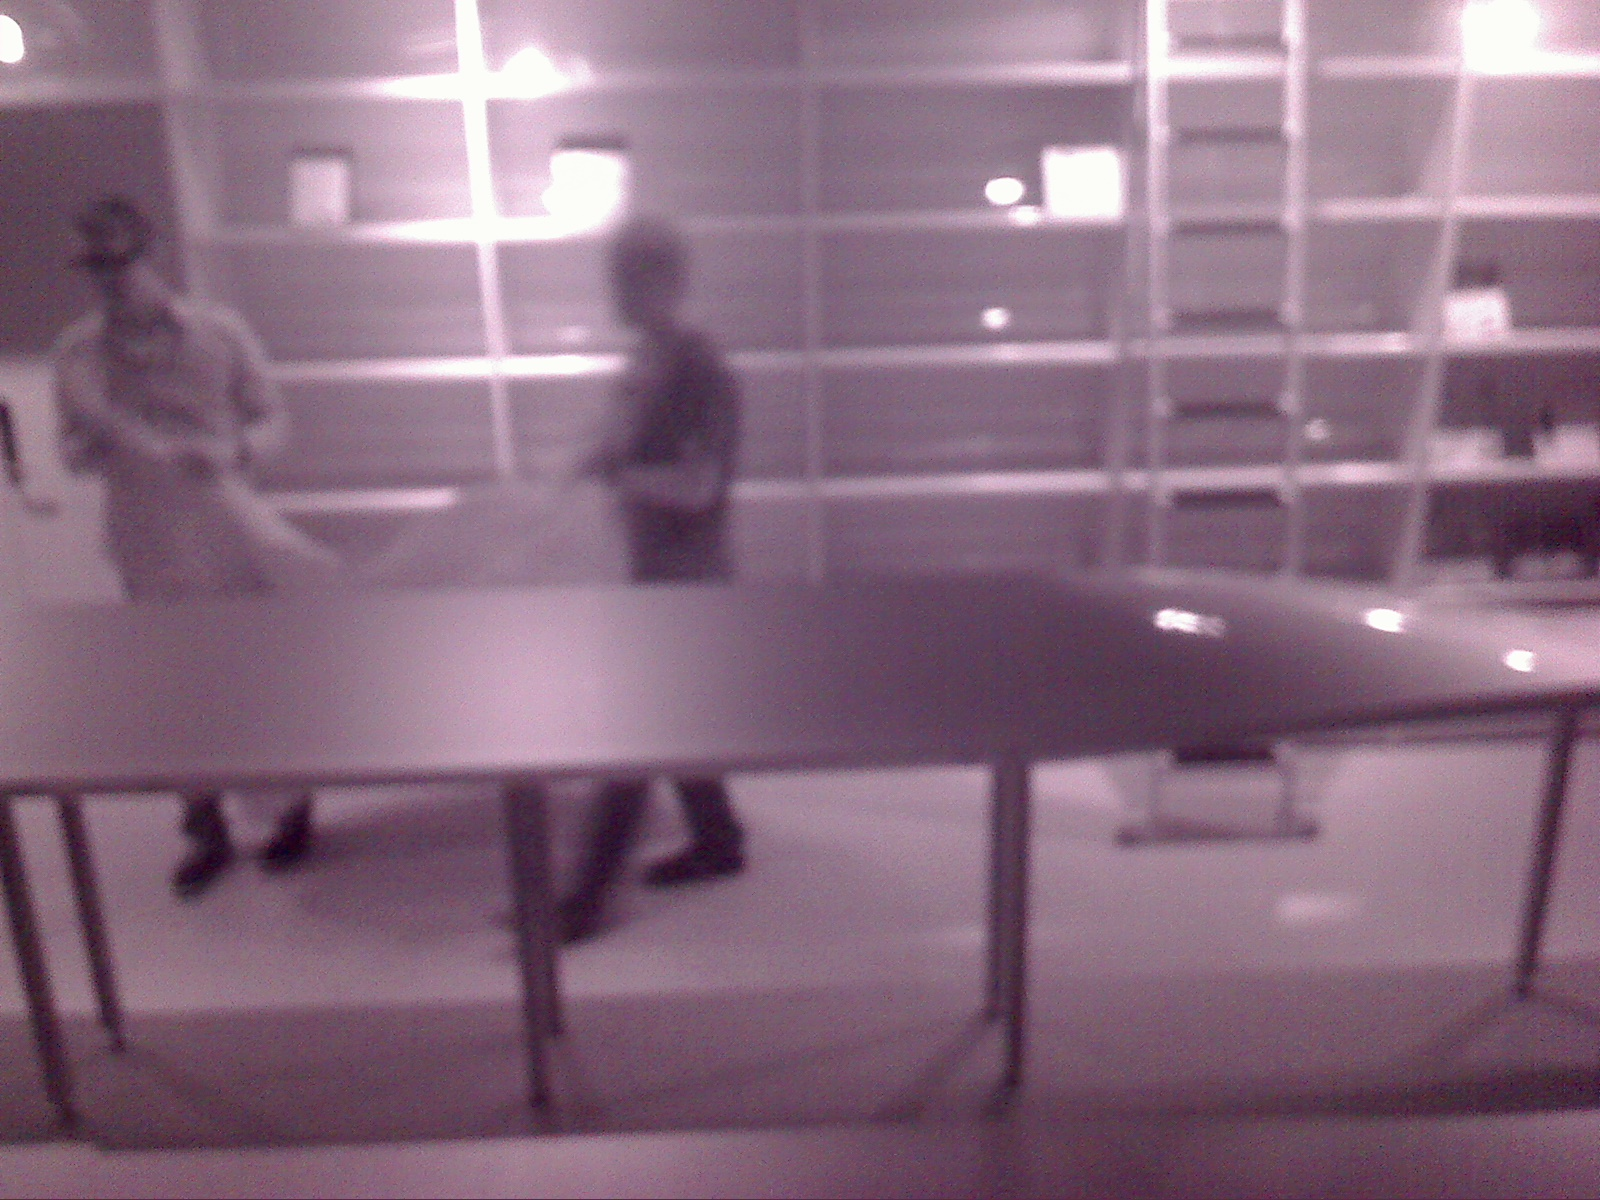
\includegraphics[width=0.7\textwidth]{Pictures/Design/ir_max}
\caption{Image seen from the IR camera.}
\label{fig:ir_max}
\end{figure}

Another possibility would have been to put all the color channels together with different weight factors, like in the conversion from a color image to grayscale image. It was chosen not to do this, because the color channels were so similar that it wouldn't have improved the final result, and it would have meant that we had to read all color channels, making the program slower. 

\subsection{Optimizing the code}\label{forInOne}
Having the previous sections in mind, we are now interested in the pixels inside the ROI that have become darker in comparison to the reference picture. Also, we would like to have the steps of reading all the pixels using OpenCV removed. This can all be written in code in a simple way, using fewer steps than needed before:

\begin{lstlisting}
void Picture::refreshDiscradBGSubtractAndThreshholdForBnW(VideoCapture captureToStoreCamra, Picture refPicture, int threshhold, int procentOfScreenUsed, int heightOfLowerROI)
{
	captureToStoreCamra >> tmp; //(1)
	for(int x = 0; x < width; x++) //(2)
	{
		for(int y = heightOfLowerROI; y > heightOfLowerROI - (int)(((float)(procentOfScreenUsed/2)/100)*height); y--)//(2)
		{
			if((int)tmp.at<Vec3b>(y,x)[2] - refPicture.pixelR[x][y] < -1*threshhold) //(3)
			{
				pixelR[x][y] = 255; //(4)
			}
			else
			{
				pixelR[x][y] = 0; //(5)
			}
		}
	}
}
\end{lstlisting}
This function does four things, as described previously: reading in pixel values with help from OpenCV; doing thresholding; using the region of interest to discard unnecessary data; and background subtraction.

\textbf{refreshDiscradBGSubtractAndThreshholdForBnW()} refreshes the picture, looking just at the region of interest, and performs calculations that provides the same result by using background subtraction and threshholding.

The first thing the function does is that it streams the current picture from the camera to a temporary \textbf{Mat} object called \textbf{tmp} (1). The next thing it does is that it loops through all the X values of the picture and through all the Y values that we are interested in (2). The Y values we are interested in are the ones that go from \textbf{heightOfLowerROI}, which is a parameter to the function, up to a specific percentage of the screen. For each of these coordinates the program checks if the red channel of the of the new picture is darker than the threshold value (3). If this is the case, the current pixel gets the maximum value, to show that this pixel has changed in comparison to the reference picture (4). If it hasn't changed enough, the pixel's value is set to to zero (5).

\begin{figure}[htbp]
\centering
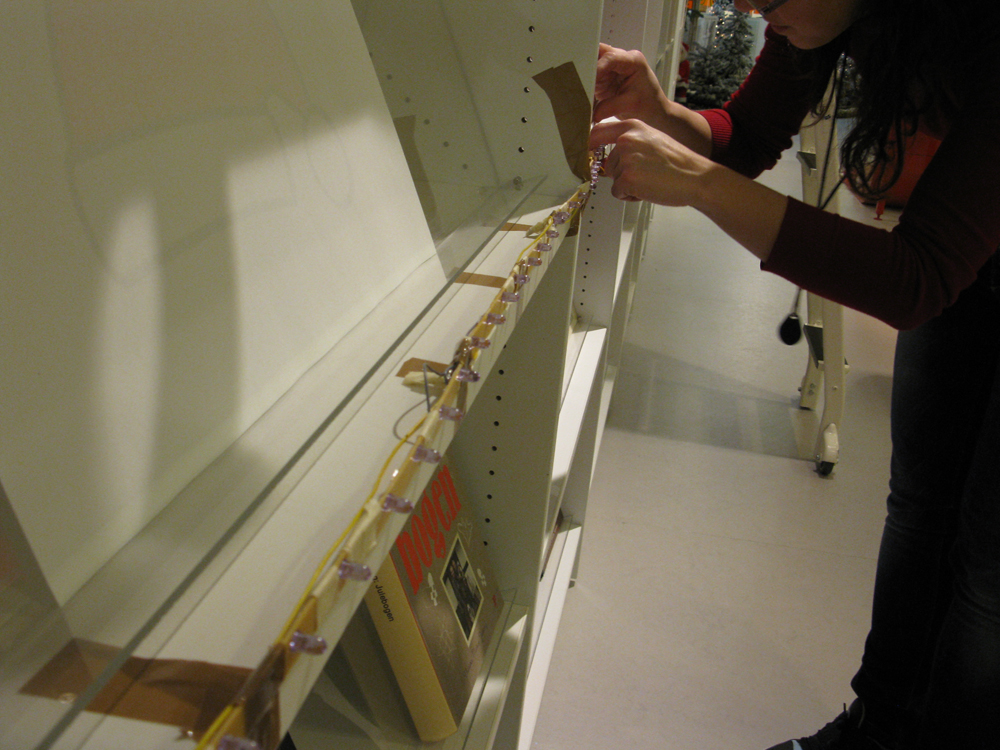
\includegraphics[width=0.7\textwidth]{Pictures/Design/led_max}
\caption{The LEDs are put on a long strip at 4 centimetres intervals.}
\label{fig:led_max}
\end{figure}

\section{Morphology}
Because the group arranged the LEDs on a long strip in an interval of 4 centimetres (see figure \ref{fig:led_max}), there were some light gaps on the taken picture. This meant that some of the pixels that actually should have been detected as changed were detected as unchanged. This caused the program to detect some persons doubled, because they were separated, even though there was in fact only a single person in front of the camera.

The group solved this by applying morphology to the picture. Closing was applied to close the gaps within the persons. As mentioned in \ref{closing}, it consist of first dilating the picture and then eroding it. This is shown in the following code:

\begin{lstlisting}
void Picture::dilate(int radius, Picture &tmpPicture)
{
	for(int x = radius; x < width-radius; x++) //(1)
	{
		for(int y = radius; y < height-radius; y++) //(1)
		{
			bool pixelIsaccepted = false;
			for(int filterX = x - radius; !pixelIsaccepted && filterX <= x + radius; filterX++) //(2)
			{
				for(int filterY = y - radius; !pixelIsaccepted && filterY <= y + radius; filterY++) //(2)
				{
					if (pixelR[filterX][filterY] == 255)(3)
					{
						pixelIsaccepted = true;
					}
				}
			}
			if (pixelIsaccepted == true)
				tmpPicture.pixelR[x][y] = 255; //(5)
			else
				tmpPicture.pixelR[x][y] = 0;
		}
	}
	for(int x = 0; x < width; x++)
		for(int y = 0; y < height; y++){
			pixelR[x][y] = tmpPicture.pixelR[x][y];
			pixelG[x][y] = tmpPicture.pixelR[x][y];
			pixelB[x][y] = tmpPicture.pixelR[x][y];
		} //(6)
}
void Picture::erode(int radius, Picture &tmpPicture)
{
	for(int x = radius; x < width-radius; x++) //(1)
	{
		for(int y = radius; y < height-radius; y++) //(1)
		{
			bool pixelIsaccepted = true;
			for(int filterX = x - radius; pixelIsaccepted && filterX <= x + radius; filterX++) //(2)
			{
				for(int filterY = y - radius; pixelIsaccepted && filterY <= y + radius; filterY++) //(2)
				{
					if (pixelR[filterX][filterY] == 0)(4)
					{
						pixelIsaccepted = false;
					}
				}
			}
			if (pixelIsaccepted == true)
				tmpPicture.pixelR[x][y] = 255; //(5)
			else
				tmpPicture.pixelR[x][y] = 0;
		}
	}
	for(int x = 0; x < width; x++)
		for(int y = 0; y < height; y++)
		{
			pixelR[x][y] = tmpPicture.pixelR[x][y];
			pixelG[x][y] = tmpPicture.pixelR[x][y];
			pixelB[x][y] = tmpPicture.pixelR[x][y];
		} //(6)
}

\end{lstlisting}
Both the erosion and dilation go through almost all the pixels in the picture. The pixels that are not analyzed are the ones that are too close to the edge of the picture, so the kernel would be empty for some of the values (1). There is various ways to circumvent this edge problem, but it was decided not to pursue these, since the pixel edges are not so important for the program, especially since the final output image will show something completely different thanks to Unity (more about this in \ref{unityStart}).

At every pixel, the functions look around the given pixel with the chosen radius (2). The difference between the \textbf{erosion()} and \textbf{dilation()} is that for a pixel to be accepted in dilation, just a single pixel in the radius has to be true (3). With erosion, there can't be any pixels in the radius that are false (4). Other than that the two functions work the same way. While the program is still looking through the image, the output has to be stored in a buffer picture. This buffer picture holds the output, so the the original input picture is left intact (5). When the functions are finished with analyzing the picture, the output from the buffer picture gets written to the picture that the function is called from (6). 

\section{The setup loop}
\subsection{Take a background picture}\label{backgroundConfig}
Like mentioned before in \ref{program_structure}, there is also a loop in the setup. This loop contains a while loop that has \textbf{true} as its condition. The loop is not supposed to end when the Escape key is pressed, but when it has figured out that there are no people in the picture. The reason for this is that it has to take a reference picture, which is the one used in the background subtraction.

The function works under the assumption that people in front of the camera always move a little and aren't standing 100\%. The function has three thresholds. The first threshold is called \textbf{threshholdPixelChange} and is the value from which a pixel can be counted as changed.

The second is \textbf{threshholdPixelsChanged} which is the threshold for how many pixels count as a person, since we are not interested if just a single pixel has changed.

The third threshold, \textbf{threshholdFramesChanged}, is set in case that a person should accidentally stand still for one frame. This threshold sets how many pictures in a row that have to taken without changes, so we can assume that nobody is on the picture. 
\begin{lstlisting}
void configBG(Picture &BG, VideoCapture &camera1, int threshholdPixelChange, int threshholdPixelsChanged, int threshholdFramesChanged, int lroi)
{
	Picture test1;
	Picture test2;
	test1.initialize(camera1);
	test2.initialize(camera1); // (1)

	double framesUnchangeged = 0; //(2)
	while(true)
	{
		test1.refresh(camera1);
		waitKey(30);
		test2.refresh(camera1); //(3)
		double pixelChange = 0; // (4)
		double pixelsChanged = 0; // (5)
		

		for(int x = 0; x < test1.width; x++)
		{
			for(int y = 0; y < test1.height; y++) // (6)
			{
				pixelChange = 0;
				if(test1.pixelR[x][y] - test2.pixelR[x][y] > 0)
					pixelChange += test1.pixelR[x][y] - test2.pixelR[x][y];
				else
					pixelChange += test2.pixelR[x][y] - test1.pixelR[x][y];

				if(test1.pixelG[x][y] - test2.pixelG[x][y] > 0)
					pixelChange += test1.pixelG[x][y] - test2.pixelG[x][y];
				else
					pixelChange += test2.pixelG[x][y] - test1.pixelG[x][y];

				if(test1.pixelB[x][y] - test2.pixelB[x][y] > 0)
					pixelChange += test1.pixelB[x][y] - test2.pixelB[x][y];
				else
					pixelChange += test2.pixelB[x][y] - test1.pixelB[x][y]; // (7)
					
				if(pixelChange > threshholdPixelChange)
					pixelsChanged++; // (8)
			}
		}
		if(pixelsChanged < threshholdPixelsChanged)
			framesUnchangeged++; // (9)
		else
			framesUnchangeged = 0; // (10)

		if(framesUnchangeged >= threshholdFramesChanged) //(11)
		{
			BG.refresh(camera1); //(12)
			int brightestYProduct = 0;
			for(int x = 0; x < BG.width; x++) //(13)
			{
				int brightestVal = 0;
				for(int y = 0; y < BG.height; y++) //(13)
				{
					if(BG.pixelR[x][y] > brightestVal)
					{
						brightestVal = BG.pixelR[x][y];
						brightestYatX[x] = y; //(14)
					}
				}
				brightestYProduct += brightestYatX[x]; //(15) 
			}
			startHeightOfROI = brightestYProduct/BG.width + BG.height*((float)procentOfTheScreenUsed/100)/4; //(16)

			if(startHeightOfROI > BG.height-1)
				startHeightOfROI = BG.height-1; //(17)
			return;
		}
	}
}
\end{lstlisting}
Before starting the while loop, \textbf{configBG()} configures the background; initializes two pictures (1); as well as a variable that will hold the number of frames that are unchanged in a row (2).

In the while loop it refreshes the pictures with a time delay of 30 milliseconds (3), and it initializes a counter that holds how much each pixel is changed (4). It also has a variable that knows how many pixels that have been changed (5). After this the program goes through all pixel coordinates (6) and saves the difference between the pixel value of each channel in the variable \textbf{pixelChange} (7).

When \textbf{pixelChange} is bigger than the threshold that classifies a pixel as being changed, the counter \textbf{pixelsChanged} gets raised by one (8). When all the pixels have been looked through, the program knows how many pixels have been changed. When sufficiently few pixels have changed, which is set by the parameter \textbf{threshholdPixelsChanged}, the counter for frames that haven't changed gets counted up(9). When to many pixels have changed the counter gets set to zero (10).
 
When enough pictures have been unchanged, the last part of the loop is entered (11). Here, first the  \textbf{Picture} object called \textbf{BG} gets refreshed (12). When this is done, we analyze two things on the picture. The first one is finding the brightest pixel's position in each column of the picture. The second is placing the region of interest. We find the brightest pixel by going through each pixel of each column (13). The brightest pixels ant their values are then stored (14). This gets saved in the integer array \textbf{brightestYatX[X]}. When feeding in an X value, it returns the Y position of the brightest pixel at that X position.

To find out where the region of interest has to be placed, the program adds all Y positions of the brightest pixels (15) together and finds the average of them in the end (16). In the end there is a check that makes sure that the region of interest is in the frame (17).

\subsection{The enter zone}
Now the question might be why we are interested in the position of the brightest pixel in each column on the background picture. The answer to that is that when a person goes into the picture and produces pixels that have been changed in comparison to the background, the person will do that in front of the LEDs. If we are looking for this person, we don't want to look through all the pixels but only the ones where the LEDs are on the background picture. We are looking for the brightest pixel, because we hope to find the pixel at the position of each LED. We will come back to this \ref{findPerson}.

\section{Finding and analysing the BLOBs}
Let's assume that we have examined a pixel that is found to be true or in other words changed in comparison to the background. The next thing would be to find the pixels that are connected to this single pixel, categorizing them as one object, also known as a BLOB (Binary Large Object). One method that is often used is recursion. That's why a recursive function, when called, could go from pixel to pixel and call itself:
\begin{lstlisting}
void Picture::startFire(point startingPoint, Picture &tmpPicture)
{
	tmpPicture.makeBlack();
	findNextPoint(startingPoint, tmpPicture);
	for(int x = 0; x < width; x++){
		for(int y = 0; y < height; y++){
			if(tmpPicture.pixelR[x][y] == 255){ 
				//pixelR[x][y] = 0;
				pixelG[x][y] = 150;
				//pixelB[x][y] = 0;
			}
		}
	}
}
void Picture::findNextPoint(point currentPosition, Picture &tmpPicture)
{
	tmpPicture.pixelR[currentPosition.x][currentPosition.y] = 255;
	//if right is available, is free and not burned
	if(currentPosition.x+1 < width && pixelR[currentPosition.x+1][currentPosition.y] == 255 && tmpPicture.pixelR[currentPosition.x+1][currentPosition.y] != 255)
		{
			//cout << "right\n";
			findNextPoint(point(currentPosition.x+1,currentPosition.y), tmpPicture);
		}
	//if down is available, is free and not burned
	if(currentPosition.y+1 < height && pixelR[currentPosition.x][currentPosition.y+1] == 255 && tmpPicture.pixelR[currentPosition.x][currentPosition.y+1] != 255)
		{
			//cout << "down\n";
			findNextPoint(point(currentPosition.x,currentPosition.y+1), tmpPicture);
		}
	//if left is available, is free and not burned
	if(currentPosition.x-1 > 0 && pixelR[currentPosition.x-1][currentPosition.y] == 255 && tmpPicture.pixelR[currentPosition.x-1][currentPosition.y] != 255)
		{
			//cout << "left\n";
			findNextPoint(point(currentPosition.x-1,currentPosition.y), tmpPicture);
		}
	//if up is available, is free and not burned
	if(currentPosition.y-1 > 0 && pixelR[currentPosition.x][currentPosition.y-1] == 255 && tmpPicture.pixelR[currentPosition.x][currentPosition.y-1] != 255)
		{
			//cout << "up\n";
			findNextPoint(point(currentPosition.x,currentPosition.y-1), tmpPicture);
		}
}
\end{lstlisting}
This function works just on smaller BLOBs. The problem was that for each pixel a new function was called causing a stack overflow. A stack overflow occurs when too much memory is used on the call stack and often results in the program crashing.

That is why there was a need to write a new function that wouldn't call itself multiple times, since it would make the program unstable and in the end stop working. To get a better overview, the logic behind behind the recursive function was written down on paper to be analyzed.

This lead to a reformulation of the logic, making the function non-recursive. However, it kept the same functionality, just in a while loop with eight cases for where the function should look next.

The first four cases are the ones where the function goes forward to the next pixel, with a priority for each direction. The priorities five to eight are for when the function already has tried to move forward and the only possibility is to go back. When none of these cases occur, the function is done with the analysis and the while loop is exited, as it is shown in the following code:
\begin{lstlisting}
void Picture::startFireLoggingPersons(point startingPoint)
{
	if(pixelR[startingPoint.x][startingPoint.y] != 255) //(7)
		return;
	//R is for Input - 255 = blob not classified, 0 = nothing found or to small
	//G is for way back

	resetChannelsExcept('R'); //function that sets all values pixel values to zero besides the one from the red channel
	point currentPosition = startingPoint; // (8)
	int pixelCount = 0; //(1)

	p[currentPersonId].minX = height + 100;
	p[currentPersonId].maxX = -100;
	
	while(true)
	{
		if(currentPosition.x > p[currentPersonId].maxX)
			p[currentPersonId].maxX = currentPosition.x;
		if(currentPosition.x < p[currentPersonId].minX)
			p[currentPersonId].minX = currentPosition.x; //(11)
					
		pixelR[currentPosition.x][currentPosition.y] = 200 + currentPersonId;

		//if right is available, is free and not burned
		if(currentPosition.x+1 < width && pixelR[currentPosition.x+1][currentPosition.y] == 255) //(3)
		{
			pixelCount++; //(9)
			pixelG[currentPosition.x][currentPosition.y] = pixelCount; //(2)
			currentPosition.x++; //(6)

		}
		//if down is available, is free and not burned
		else if(currentPosition.y+1 < height && pixelR[currentPosition.x][currentPosition.y+1] == 255) //(3)
		{
			pixelCount++; //(9) 
			pixelG[currentPosition.x][currentPosition.y] = pixelCount; //(2)
			currentPosition.y++; //(6)
		}
		//if left is available, is free and not burned
		else if(currentPosition.x-1 >= 0 && pixelR[currentPosition.x-1][currentPosition.y] == 255) //(3)
		{
			pixelCount++; //(9)
			pixelG[currentPosition.x][currentPosition.y] = pixelCount; //(2)
			currentPosition.x--; //(6)
		}
		//if up is available, is free and not burned
		else if(currentPosition.y-1 >= 0 && pixelR[currentPosition.x][currentPosition.y-1] == 255) //(3)
		{
			pixelCount++; //(9)
			pixelG[currentPosition.x][currentPosition.y] = pixelCount; //(2)
			currentPosition.y--; //(6)
		}
		//steps back:
		//if right is available, burned and has the biggest count(also check if the pixel, that is compared to is available) -> we have been there last -> go back 
		else if(currentPosition.x+1 < width && (currentPosition.y+1 >= height || pixelG[currentPosition.x+1][currentPosition.y] > pixelG[currentPosition.x][currentPosition.y+1]) && (currentPosition.x-1 < 0 || pixelG[currentPosition.x+1][currentPosition.y] > pixelG[currentPosition.x-1][currentPosition.y]) && (currentPosition.y-1 < 0 || pixelG[currentPosition.x+1][currentPosition.y] > pixelG[currentPosition.x][currentPosition.y-1])) //(4)
		{
			pixelG[currentPosition.x][currentPosition.y] = 0; //(5)
			currentPosition.x++; //(6)
		}
		//if down is available, burned and has the biggest count -> we have been there last
		else if(currentPosition.y+1 < height && (currentPosition.x+1 >= width || pixelG[currentPosition.x][currentPosition.y+1] > pixelG[currentPosition.x+1][currentPosition.y]) && (currentPosition.x-1 < 0 || pixelG[currentPosition.x][currentPosition.y+1] > pixelG[currentPosition.x-1][currentPosition.y]) && (currentPosition.y-1 < 0||pixelG[currentPosition.x][currentPosition.y+1] > pixelG[currentPosition.x][currentPosition.y-1])) //(4)
		{
			pixelG[currentPosition.x][currentPosition.y] = 0; //(5)
			currentPosition.y++; //(6)
		}
		//if left is available, burned and has the biggest count -> we have been there last
		else if(currentPosition.x-1 >= 0 && (currentPosition.y+1 >= height || pixelG[currentPosition.x-1][currentPosition.y] > pixelG[currentPosition.x][currentPosition.y+1]) && (currentPosition.x+1 >= width || pixelG[currentPosition.x-1][currentPosition.y] > pixelG[currentPosition.x+1][currentPosition.y]) && (currentPosition.y-1 < 0 || pixelG[currentPosition.x-1][currentPosition.y] > pixelG[currentPosition.x][currentPosition.y-1])) //(4)
		{
			pixelG[currentPosition.x][currentPosition.y] = 0; //(5)
			currentPosition.x--; //(6)
		}
		//if up is available, burned and has the biggest count -> we have been there last
		else if(currentPosition.y-1 >= 0 && (currentPosition.x+1 >= width || pixelG[currentPosition.x][currentPosition.y-1] > pixelG[currentPosition.x+1][currentPosition.y]) && (currentPosition.x-1 < 0||pixelG[currentPosition.x][currentPosition.y-1] > pixelG[currentPosition.x-1][currentPosition.y]) && (currentPosition.y+1 >= height||pixelG[currentPosition.x][currentPosition.y-1] > pixelG[currentPosition.x][currentPosition.y+1])) //(4)
		{
			pixelG[currentPosition.x][currentPosition.y] = 0; //(5)
			currentPosition.y--; //(6)
		}
		else
			break;
	}
	
	if(pixelCount > minPixelToBeAPerson) //(10)
	{
		float average = ((p[currentPersonId].minX + p[currentPersonId].maxX)/2); //(12)
		float zeroToOne = average/width;
		p[currentPersonId].posX = zeroToOne;
	}
	else //(10)
		for(int y = 0; y < height; y++)
			for(int x = 0; x < width; x++)
				if(pixelR[x][y] ==  200 + currentPersonId;)
					pixelR[x][y] = 0;
		p[currentPersonId].posX = -1;
	}
}
\end{lstlisting}
This is the function that replaced our previous recursive function.

It somehow violates the pixel system we had until then. The different channels are not used to saving the color channels of the picture any longer. Instead, the states of the analysis of the pixels are saved in the color channels. When the red channel of the pixel has a value of 255, the pixel is found but not yet analyzed by the function. When it is 0, it means that nothing is found, and when it is another number, it is going to be analyzed.

One can find the BLOB index number, as well as which pixel it belongs to, by subtracting 200 from its value. The blue channel isn't used. The green channel is used to save the way that function goes with the four first forward-cases, so it in the following four cases knows which way the way back is. The function does that by counting the pixels with the \textbf{pixelCount} (1). The count is assigned to the green channel of every pixel that is found forwards (2). When non of the four if statements (3) have become true, the function compares the counter in the green values around itself and goes to the biggest; in other words finds the position where it has been last (4). In order to not let the function go there again the green channel is set to zero, when going backwards(5).

The function move through the pixels in all eight cases and updating the object \textbf{currentPosition}, which is a struct of type \textbf{point}. This struct contains two integers called \textbf{X} and \textbf{Y}. When the object move in a direction, X or Y are either increased or reduced (6).

After that, the while loop runs with the new given position. When calling the function, one has to put in the point where the function will start to analyze the BLOB, in this case called \textbf{startingPoint}. The starting point will in the beginning of the function be checked if it is found to be 255 in the red channel (7) and then be set to the \textbf{currentPosition} (8). While going through the BLOB, the function also saves some information about it: it counts how many pixels the BLOB consists of (9). We use this information to discard BLOBs that are too small to be considered as a person (10). If this is the case, the \textbf{personCounter} gets reset to what it was before the function was called, and the pixel values are set to zero. The function also saves the biggest and  smallest X positions of the BLOB (11). In case the \textbf{personCounter} is big enough, the average of these two number is stored in the \textbf{posX} and is later used to output where the person is positioned in front of the screen (12).

\section{Persons}
Now it is possible categorize the pixels in BLOBs and assign them a number. The next question was how to keep track of where each person went from frame to frame. When we just would go through the whole picture in every frame, the BLOBs would always be numbered in the order they were found, from the upper left corner to the lower right corner.

It was decided that the persons found in the picture should be stored in an array of found persons. From frame to frame, the persons would then have to be re-found, so there was a connection between the person from the previous frame to the current frame. It was important that the program first would try to re-find the persons, and then it would look for new persons among the BLOBs that hasn't been touched yet.

Another thing to be considered was when people should be allowed to enter the picture, and what should happen if a person from one frame to the next disappeared. Was it likely that the person reached the edge of the picture and then walked out of it? There was also a possibility for that the person was occluded, i.e. hidden, by another person. How to separate this case from the case of exiting the picture?

Here we will at first describe how a person is stored in the program, secondly how it is found in the beginning, and then how it is re-found. We structure it like this, even though in the main loop we first try to re-find the person and then look for new persons.

\subsection{The person class}
When choosing how to keep track of the person that has already been found, the group decided to make a new class called \textbf{person}. This person class was decided to be a member of the \textbf{Picture} class. 
\begin{lstlisting}
class Picture
{
public:
	
	class person
	{
	public:

		float posX; //(1)
		int minX; //(2)
		int maxX; //(3)
		float moveVector; //(4)
		int heightOfROI; //(5)
		double id; //(6)
		int pId; //(7)

		bool notAddedToTheNewInitialMoveVectorProductYet; //(8)

		bool refind(Picture& parent); //(9)
		bool refindOccluded(Picture& parent);//(10)

	}p[50]; //(8)
	{...}
}
\end{lstlisting}
The \textbf{moveVector} (4) is the vector with which the person has moved from the last frame to the current frame. This vector has just one dimension. The \textbf{heightOfROI} (5) is a variable that should hold the height of the region of interest where the person was found. The \textbf{id} (6) is the id tag that describes where the person stepped into the picture. For instance, the person number 221 to step into the picture after the program had been launched would get the id 221.

Then there is \textbf{pId} (7), which is each person's id number in their own array. This array is also a member of the \textbf{Picture} class (8). The array allows for a maximum of 50 people, and since it is zero-based, \textbf{pId} is always between 0 and 49.

\subsection{Finding new persons}\label{findPerson}
When trying to find new persons, the group limited the search to looking at the left-most and the right-most pixels, since nobody could come from above or from the underneath the camera.

Since they also limited it to a region of interest, they also just had to look for new persons in this area. It was decided to only look at the brightest pixel where, hopefully, the LED strip was positioned.

\begin{lstlisting}
void Picture::lookForNewPersons(int procentOfScreenUsedForEnterAndExit, int brightestYatX[])
{
		for(int x = 0; x < width * (procentOfScreenUsedForEnterAndExit/2) / 100; x++) //(1)
		{
			if(pixelR[x][brightestYatX[x]] == 255)  //(2)
			{ 
				point currentPoint;
				currentPoint.x = x;
				currentPoint.y = brightestYatX[x];

				int j = 0;
				do
				{
					currentPersonId = j;
					j++;
				} 
				while (j < 51 && p[j-1].posX != -1); //(3)

				startFireLoggingPersons(currentPoint); //(4)

				if(p[currentPersonId].posX != -1) //(5)
				{
					personCount++; //(6)
					p[currentPersonId].id = personCount; //(7)
					
					p[currentPersonId].notAddedToTheNewInitialMoveVectorProductYet = true;
					p[currentPersonId].moveVector = initialMoveVector;
					p[currentPersonId].heightOfROI = brightestYatX[x]; //(8)
				}
			}
		}
		for(int x = width-1; x > width - ((width * (procentOfScreenUsedForEnterAndExit/2)) / 100); x--) //(1)
		{
			if(pixelR[x][brightestYatX[x]] == 255) //(2)
			{
				point currentPoint;
				currentPoint.x = x;
				currentPoint.y = brightestYatX[x];

				int j = 0;
				do
				{
					currentPersonId = j;
					j++;
				} 
				while (j < 51 && p[j-1].posX != -1); //(3)

				startFireLoggingPersons(currentPoint); //(4)

				if(p[currentPersonId].posX != -1) //(5)
				{
					personCount++; //(6)
					p[currentPersonId].id = personCount; //(7)
					
					p[currentPersonId].notAddedToTheNewInitialMoveVectorProductYet = true;
					p[currentPersonId].moveVector = -1*initialMoveVector;
					p[currentPersonId].heightOfROI = brightestYatX[x]; //(8)
				}
			}
		}
}
\end{lstlisting}
When calling this function, one has to put in how many percentages of the screen one wants to use for the enter zone (the zone where new persons are allowed to enter the picture). These percentages refer to the percent of the X axis that should be used.

The program then loops through the relevant X values in two for loops (1). The array of the brightest Y values is used in combination with the X value to find the position where we want to look for a new person. When the red channel of the pixel is 255, meaning that it is found by in preprocessing part, but not yet analyzed, the program starts to analyze the BLOB (2). This is done by first finding a \textbf{person} object in the array that is empty, by looking for one which X position is -1 (3). -1 is the value that is given to all \textbf{person} objects initially, and when they disappear. After that the function \textbf{startFireLoggingPersons()} is called(4). Since an empty \textbf{person} object was found, the \textbf{startFireLoggingPersons()} function fills the empty \textbf{person}. unless the BLOB is too small. When the BLOB is too small, the \textbf{person} gets the status of being empty; this is done by setting its \textbf{posX} to -1 again.

When the function \textbf{startFireLoggingPersons()} is called, and the \textbf{posX} is not -1 (5), the \textbf{person} counter gets increased by one (6), and the person's id is  set to the corresponding value (7). Furthermore, \textbf{notAddedToTheNewInitialMoveVectorProductYet} is set to true, and \textbf{moveVector} is set to an initial value, since the person did not exist one frame ago.

In the next sections we will describe how we find the pre-found persons, as well as describing \textbf{moveVector}. Finally, the Y value in which the BLOB was found gets saved in the \textbf{heightOfROI} (8).

\subsection{Re-finding a previous-found person}
When trying to find a BLOB again, there are different approaches one can use. An often-used method is to analyze the BLOB and save specific data of it, so it can be recognized in the next frame again. Here, one could for example use the color or the shape of the object. In the case of the chosen setup, this wasn't really possible, due to the fact that the group chose to filter all the visible light out and just collect the infrared light.

This makes all the color informations disappeared. Also, almost all the information about the shape get discarded, since the camera just looks at a small strip of LEDs. This does just tell us the position of the BLOB in the X axis. By combining the current X position with one or more previous X positions, one can predict the movement that the BLOB will take on the X axis, and by that establish a connection between the BLOBs from frame to frame. 

The following approach of predicting movement is inspired by \citep{motion_move}.

The methods are highly dependent on the continuity of movement. The movement of BLOBs are predicted by looking at how the BLOB moved from the previous frame to the current frame. This is saved in a move vector. The theory is that when the move vector is added to the current position again, then we will get the new position.
 
When the program shouldn't find anything at this point, it was assumed that the object would have stopped moving. So this is the next thing that is checked. If this isn't the case, the program takes the midpoint of these two points and move to the edges until a maximum distance to move is reached. 
\begin{lstlisting}
bool Picture::person::refind(Picture& parent)
{
	point currentPoint;
	bool found = false;
	int maxAmountToMove = parent.maxAmountToMove;
	parent.currentPersonId = pId;

	if(posX+moveVector < 1 && posX+moveVector >= 0 && parent.pixelR[(int)((posX+moveVector)*parent.width)][heightOfROI] == 255) //(1)
	{
		//first priority to look is the position+the move vector (has moved normal)
		currentPoint.x = (int)((posX+moveVector)*parent.width);
		currentPoint.y = heightOfROI;
		parent.startFireLoggingPersons(currentPoint); //(6)
		if(parent.p[parent.currentPersonId].posX != -1) //(7)
		{
			cout << "found first try \n";
			found = true; //(8)
		}
	} 
	if(posX < 1 && posX >= 0 && parent.pixelR[(int)(posX*parent.width)][heightOfROI] == 255 && !found) //(2)
	{
		//second priority to look is the position (has stoped)
		currentPoint.x = (int)(posX*parent.width);
		currentPoint.y = heightOfROI;
		parent.startFireLoggingPersons(currentPoint); //(6)
		if(parent.p[parent.currentPersonId].posX != -1) //(7)
		{
			cout << "found second try \n";
			found = true; //(8)
		}
	} 
	//third priority is to look around the most likely point until the max amount to move is reached
	for(int i = 0; (int)((moveVector/2)*parent.width)+i <= maxAmountToMove && (int)((moveVector/2)*parent.width)-i >= -maxAmountToMove && !found; i++) //(3)
	{
		if((int)((posX+moveVector/2)*parent.width)+i < parent.width && (int)((posX+moveVector/2)*parent.width)+i >= 0 && parent.pixelR[(int)((posX+moveVector/2)*parent.width)+i][heightOfROI] == 255) //(4)
		{
			currentPoint.x = (int)((posX+moveVector/2)*parent.width)+i;
			currentPoint.y = heightOfROI;
			parent.startFireLoggingPersons(currentPoint); //(6)
			if(parent.p[parent.currentPersonId].posX != -1) //(7)
			{
				cout << "found normal \n";
				found = true; //(8)
				break; //(9)
			}
		}
		if((int)((posX+moveVector/2)*parent.width)-i < parent.width && (int)((posX+moveVector/2)*parent.width)-i >= 0 && parent.pixelR[(int)((posX+moveVector/2)*parent.width)-i][heightOfROI] == 255) //(5)
		{
			currentPoint.x = (int)((posX+moveVector/2)*parent.width)-i;
			currentPoint.y = heightOfROI;
			parent.startFireLoggingPersons(currentPoint); //(6)
			if(parent.p[parent.currentPersonId].posX != -1) //(7)
			{
				cout << "found normal \n";
				found = true; //(8)
				break; //(9)
			}
		}
	}
	return found; //(10)
}
\end{lstlisting}
This function contains the three priorities for where we would like to look for the BLOB

First the position is checked for where the BLOB should be when it would move with a constant speed (1). The next priority is when the object has stopped abruptly (2).

The last priority is looking several places: starting from the position between the two previous points, the function goes to both sides until it on one of the side hits the border for the maximum distance to move. This is done by having a forloop that iterates  from 0 and up (3). This number is then added (4) and subtracted (5) to the midpoint of the two first points. Like when looking for new persons, the program starts the \textbf{startFireLoggingPersons()} with the point the function has found to be true (red channel is 255) (6). If this function has set the persons position to something that is not -1 (7), it will end itself by setting the boolean variable \textbf{found} to true (8), breaking the loop (9). In the end of the function it will return whether the person was found or not (10).

\subsection{Occluded or exited}
The last thing that can happen now is that the person can disappear. When a person disappears, it is because one of three reasons: the person'ss BLOB is occluded, hidden, by another BLOB (see figure \ref{fig:enterexit}); the person has exited (see figure \ref{fig:occlusion}) the picture; or the system has made an error. This logic is implemented in the main loop.

\begin{figure}[htbp]
\centering
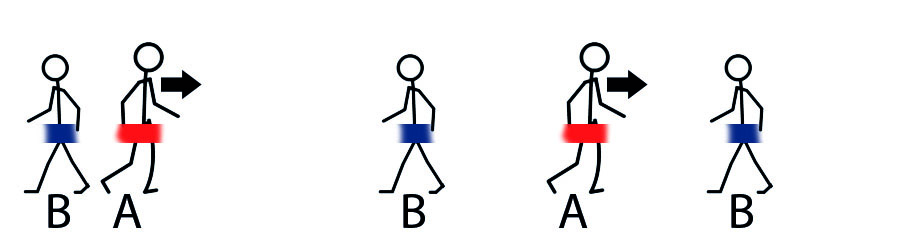
\includegraphics[width=1.00\textwidth]{Pictures/Design/enterexit.jpg}
\caption{Illustration of how person B stays in the picture, while person A exits it. The red and the blue bar show their detected BLOBs.}
\label{fig:enterexit}
\end{figure}

\begin{lstlisting}
for(int i = 0; i < maxNumberOfPersons; i++) //(1)
		{
			if(currentPicture.p[i].posX != -1) //(2)
			//the person does exist
			{
			float prePos = currentPicture.p[i].posX;  //(3)
				if(!currentPicture.p[i].refind(currentPicture))  //(4)
				{
				//new position of the person not found
				//either person is exited or occluded
					if(((prePos*currentPicture.width) - currentPicture.maxAmountToMove > 0) && ((prePos*currentPicture.width) + currentPicture.maxAmountToMove < currentPicture.width)) //(5)
					// check if the person is NOT close enogth to the edge of the picture to exit
					{
						//is not close enough to the border of the picture to exit -> it must be occluded
						if(!currentPicture.p[i].refindOccluded(currentPicture)) //(7)
						{
						//the person is not found, not occluded and not exited 
							currentPicture.p[i].posX = -1; //(8)
							cout << "Person is magical disappeared"
						}
					}
					else 
					{
					//the person is exited normally 
						currentPicture.p[i].posX = -1; //(6)
					}


					if(currentPicture.p[i].notAddedToTheNewInitialMoveVectorProductYet) //(9)
					{ 
					//when the initial movevector isn't measured yet
					
						currentPicture.newInitialMoveVectorProduct = currentPicture.initialMoveVector; //(11)
						//since there is nothing to take the average take the initial move vector from this run
					}


				}
				currentPicture.p[i].moveVector = currentPicture.p[i].posX - prePos;
				if(currentPicture.p[i].notAddedToTheNewInitialMoveVectorProductYet) //(9)
				{
					if(currentPicture.p[i].moveVector < 0)
						currentPicture.newInitialMoveVectorProduct += -currentPicture.p[i].moveVector; //(10)
					else
						currentPicture.newInitialMoveVectorProduct += currentPicture.p[i].moveVector; //(10)
				}
			}
			currentPicture.p[i].notAddedToTheNewInitialMoveVectorProductYet = false; // <- and make shure that it isn't added again
		}
\end{lstlisting}
This logic is looping through all the \textbf{person} objects of the current picture (1). At every  the program first finds out if the person was previously found, by asking if its position is not equal to -1 (2). When the person was found in the previous frame, the program saves its \textbf{posX} in a float called \textbf{prePos} (3). After that, the function that is supposed to find the previous (old) person is called in an if statement (4). If the person can't be found again, the function tests if the person is close enough to the border that it could have exited it (5). In this case the person gets removed out of the \textbf{person} array, by setting its \textbf{posX} to -1 (6).

\begin{figure}[htbp]
\centering
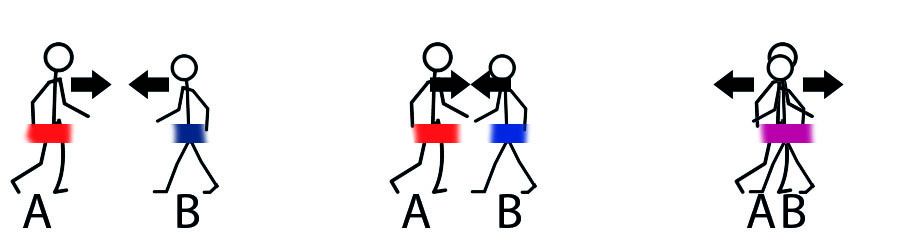
\includegraphics[width=1.00\textwidth]{Pictures/Design/occluded.jpg}
\caption{Illustration of how person B occludes Person A. The red and the blue bar show their detected BLOBs, and on the last frame their purple occluded BLOB.}
\label{fig:occlusion}
\end{figure}

If the person on the other hand is so far away that it can't exit the picture, the only logical explanation is that the person is occluded by another person. This is tested by the function \textbf{refindOccluded()}, which is positioned in a if statement like the \textbf{refind()} function (7). The \textbf{refindOccluded()} function is very similar to \textbf{refind()}, only that it looks for values that are not 0 instead of some that are 255. It also sets the \textbf{xPos} value of the occluded BLOBs equal to each other, when an occlusion is detected.
\begin{lstlisting}
bool Picture::person::refindOccluded(Picture& parent)
{
	point currentPoint;
	bool found = false;
	int maxAmountToMove = parent.maxAmountToMove;
	parent.currentPersonId = pId;

	if(posX+moveVector < 1 && posX+moveVector >= 0 && parent.pixelR[(int)((posX+moveVector)*parent.width)][heightOfROI] != 0)
	{
		//first priority to look is the position+the move vector (has moved normal)
		posX = parent.p[parent.pixelR[(int)((posX+moveVector)*parent.width)][heightOfROI]-200].posX;
		found = true;
	} 
	if(posX < 1 && posX >= 0 && parent.pixelR[(int)(posX*parent.width)][heightOfROI] != 0 && !found)
	{
		//second priority to look is the position (has stoped)
		posX = parent.p[parent.pixelR[(int)(posX*parent.width)][heightOfROI]-200].posX;
		found = true;
	} 
	for(int i = 0; (int)((moveVector/2)*parent.width)+i <= maxAmountToMove && (int)((moveVector/2)*parent.width)-i >= -maxAmountToMove && !found; i++/*check if this works*/)
	{
		if((int)((posX+moveVector/2)*parent.width)+i < parent.width && (int)((posX+moveVector/2)*parent.width)+i >= 0 && parent.pixelR[(int)((posX+moveVector/2)*parent.width)+i][heightOfROI] != 0)
		{
			posX = parent.p[parent.pixelR[(int)((posX+moveVector/2)*parent.width)+i][heightOfROI]-200].posX;
			found = true;
			break;
		}
		if((int)((posX+moveVector/2)*parent.width)-i < parent.width && (int)((posX+moveVector/2)*parent.width)-i >= 0 && parent.pixelR[(int)((posX+moveVector/2)*parent.width)-i][heightOfROI] != 0)
		{
			posX = parent.p[parent.pixelR[(int)((posX+moveVector/2)*parent.width)-i][heightOfROI]-200].posX;
			found = true;
			break;
		}
	}
	return found;
}
\end{lstlisting}
If this function also returns false, it means that there must have been a mistake with the person and that it has disappeared out of the picture (8).

\subsection{The move vector adaption}
When configuring and setting the threshold values for the program, it was often somewhat hard to find the optimal values at which the program would operate best. This was especially the case when having to say how fast the person initially moved into the frame. That's why it was decided to let the program measure how fast people are moving from the first frame to the second.

Here we have to look at the rest of the loop that goes through the persons that aren't explained yet. The idea is that when the program is running, it would take the average of the initial move vector of all the persons that have walked into the picture, and write that to a file. This file could be read the next time the program started, getting a more accurate result.

The way the average of the initial move vectors is made is that every time the person \textbf{counter} is increased, the measured actual initial move vector is added to the product of all the move vectors. For this the boolean variable \textbf{notAddedToTeInitialMoveVectorProduct}, which was set to true in the \textbf{lookForNewPersons()} function, is used. When finding a person or multiple persons again, this boolean is checked (9) and when found true, the move vector gets added (10). In most cases this works; the problem is just when a person is found and disappears in the next frame. To not to confuse the person counter system in the program, it was chosen to add the initial move vector that the program started with again (11). 

\section{Using Unity to handle the graphical output}\label{unityStart}
After doing the initial prototype, the group realized that it would be difficult to use OpenCV to both extract the data from the camera and display it in some kind of graphical way. Since the program has to loop through a lot of data continuously, there was little resources left for it to actually display the results in an interesting way without being too slow. First the group thought about using multiple threads running in the program, but even then it would be hard to display more sophisticated graphics. OpenCV is not meant as a tool to display graphics, but more to for the analyzing/extracting part.

Then the group came up with the idea of using Unity game engine to display the graphics based on the data from OpenCV. This had the added bonus of being able to use elements such as particle effects, physics and sound. Since some group members already had experience with Unity, it seemed a good choice. The only concern was how to send the data from OpenCV to Unity. OpenCV uses C++, while Unity uses \texttt{C\#}, JavaScript or Boo as scripting languages.

\subsection{Getting a link between OpenCV and Unity}
It was first considered to make C++ write to a text file that could then be read by Unity. This approach was not used in the end, since it would need a lot of readings and writings to the hard drive - doing this repeatedly could destroy it. Also, there is a chance that there would be a mismatch with Unity trying to read the file while C++ is writing to it (the text file has to be opened, then written to, and finally closed). It was also found that this method was quite slow. Therefore it was decided to write to the Clipboard in Windows.

The Clipboard acts as a short-term buffer to store temporary data in the RAM (Random Access Memory). Using copy and paste functionality, it can work like a gateway for transferring information from one program to another. \citep{clipboard_one}. This avoids writings/readings from a physical hard drive and won't wear it out, as well as being faster than saving to a text file on the computer.

\subsubsection{Copy data from C++}
In the C++ program a text line is saved as a string. This is done using the function \textbf{SetClipboardData()} where the data type has a format called CF\_TEXT that stores the data as text.\citep{clipboard_two} \citep{clipboard_three}. This string describes the information of where a person is currently located.

First it assigns an unique ID name, showing what number of person it is, and then a floating point value between 0 (left) and 0.9 (right). If it is -1, it means that the person is currently not there, i.e. there is no person. The reason for this is to make it easier for Unity to move the characters around on the screen. If a position is different from -1, it means that it should be shown on the screen. Else if the position data is -1, the character will be moved outside of the screen area and not shown.

Below is an example of the string that is copied to the Clipboard in the C++ program:

q iObject\_1p0.1 iObject\_2p0.2 iObject\_3p0.3 iObject\_4p0.4 iObject\_5p0.5 iObject\_6p0.6 iObject\_7p0.7 iObject\_8p0.8 iObject\_9p0.9 iObject\_10p-1 q

Even though the program in theory could track more people, a finite number of 10 was chosen to reduce the information used. Also, it seems unrealistic that there would be more than a total of 10 persons in front of the camera at the same time. Having this limit made it easier to handle the objects in Unity: instead of spawning a new character every time a person steps in, it just reuses the same 10 characters and move them around appropriately.

\subsubsection{Reading data in Unity}
In Unity, using \texttt{C\#}, the text is read from the Clipboard via the static function \textbf{GetSystemCopyBufferProperty()}. The first thing that happens is that whitespaces are removed. Then the string is split multiple times using different delimit characters such as the q's, i's and p's.

'q' is simply used to start and end the string, so nothing before or after is used. This was to ensure that incorrect data would never be read in Unity, i.e. if there was any leftovers from the last time data was copied to the Clipboard. It made debugging easier, since it would produce an exception error if the data in the Clipboard didn't start and end with 'q'.

The character 'i' is used to identify each person and assign it a name. In this case the name consists of a number that increases for each person that has been in front of the camera. Doing this makes it easier to identify a specific character in Unity and check if it is moving as intended. The floating value after the 'p' is the actual position of the character, which is then translated into a coordinate system in Unity where 0.1 is to the left side and 0.9 is to the right side. As mentioned before, a -1 is an invalid value, meaning that the person is not present and will therefore be moved outside of the visible screen.

In the end, all the position data are stored in an array with the position data called \textbf{Position[]}. In this case Position[0] would be the character named "Object\_1" and have the position 0.1. Position[9], on the other hand, has a -1 and would therefore not be shown on the screen.

It should be noted that these values are only for the X position. It was chosen not to use Y position to make it simpler, and since there is no depth, the Z axis is totally excluded (the program is held in 2D). However, the characters move somewhat randomly up and down in the Y direction every time the are moving around on the X direction - depending on what type of character it is. For instance, the angel character should float in the air, while the snowman should be on the ground. Doing this avoid having a lot of characters occluding each other, since more of the screen is being used (see figure \ref{fig:withoutRandomY} and \ref{fig:withRandomY}).

\begin{figure}[htbp] \centering
\begin{minipage}[b]{0.45\textwidth} \centering

\includegraphics[width=1.00\textwidth]{Pictures/Design/without_randomY} % Venstre billede
\end{minipage} \hfill
\begin{minipage}[b]{0.45\textwidth} \centering

\includegraphics[width=1.00\textwidth]{Pictures/Design/with_randomY} % Højre billede
\end{minipage} \\ % Captions og labels
\begin{minipage}[t]{0.45\textwidth}
\caption{Without random Y position.} % Venstre caption og label
\label{fig:withoutRandomY}
\end{minipage} \hfill
\begin{minipage}[t]{0.45\textwidth}
\caption{With random Y position.} % Højre caption og label
\label{fig:withRandomY}
\end{minipage}
\end{figure}

Having this array of position data makes it easy to loop through a list of Unity game objects and move them around accordingly.

Additional functionality was implemented to make the characters move more smoothly than simply jumping from point to point, which gave an effect as if they were teleporting. First of all a threshold value is used so a character will only move if the person moves enough for the system to trigger it. This means that if a person is standing still in front of the camera, the character on screen will not jump around due to the small changes in the decimal values (e.g. from 0.542 to 0.523 would not make the character move).

To make the characters move even more smoothly, it was chosen to de-synchronize the position data gathered from the camera and the character's actual position; a target system was implemented for this purpose. This works by at intervals finding a new target to move to, and then a character will gradually move towards that target. Then after a small period of time, the target will be updated. Like the threshold, it makes the characters move in a more natural line.

\subsection{Using Unity to display the characters}
The Unity game engine is typically used to make 3D games, but it is still possible to make programs in 2D, using 2D sprites/textures and an orthographic camera that doesn't display depth.

The scene used for the game is quite simple. It consists of a background image showing mountains. To achieve a more dynamic look, a couple of elements are added to make the whole scene spring to life.

First there are are a collection of Christmas trees with some Christmas balls and bells hanging on top. Using built-in physics in Unity, these bounce back and forth, simulating the wind blowing. Along with this is the falling snow, which is made as an particle system in Unity. This ensures that even when there are nobody in front of the camera, the program still feels alive.

\subsection{Time manager and Santa Claus}
As mentioned in chapter \ref{hjoerring}, the library is build on the theme of serendipity, e.g. to surprise and be new. When making the program, the group had an idea about having it change depending on the time of the day. Using the clock in Windows, the program could do something different at different times.

In the program, the sun will gradually rise as time passes, as well as the light will become brighter/dimmer, just as it is happening outside. Figures \ref{fig:time1}, \ref{fig:time2} and \ref{fig:time3} illustrate this. One thing we needed to have in mind was the light setting. On a computer screen the image can be really bright and really dark, but on a canvas and a projector it is not easy to see a dark image. Therefore the brightness level was set a little higher than normal, so it would still be possible to see it properly on the canvas. It was important to have big contrasts, so everything would look more clear on the canvas.

\begin{figure}[htbp]\centering
	\begin{minipage}[b]{0.3\textwidth}\centering
		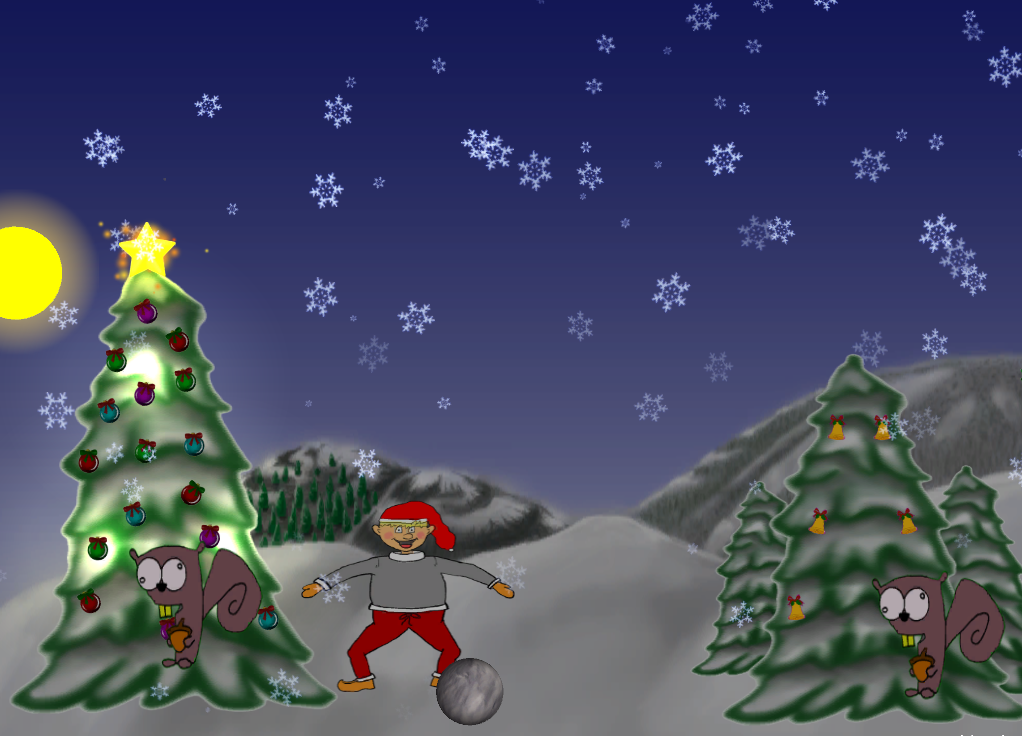
\includegraphics[width=1.00\textwidth]{Pictures/Design/time1.png} %Venstre billede
	\end{minipage}\hfill
	\begin{minipage}[b]{0.3\textwidth}\centering
		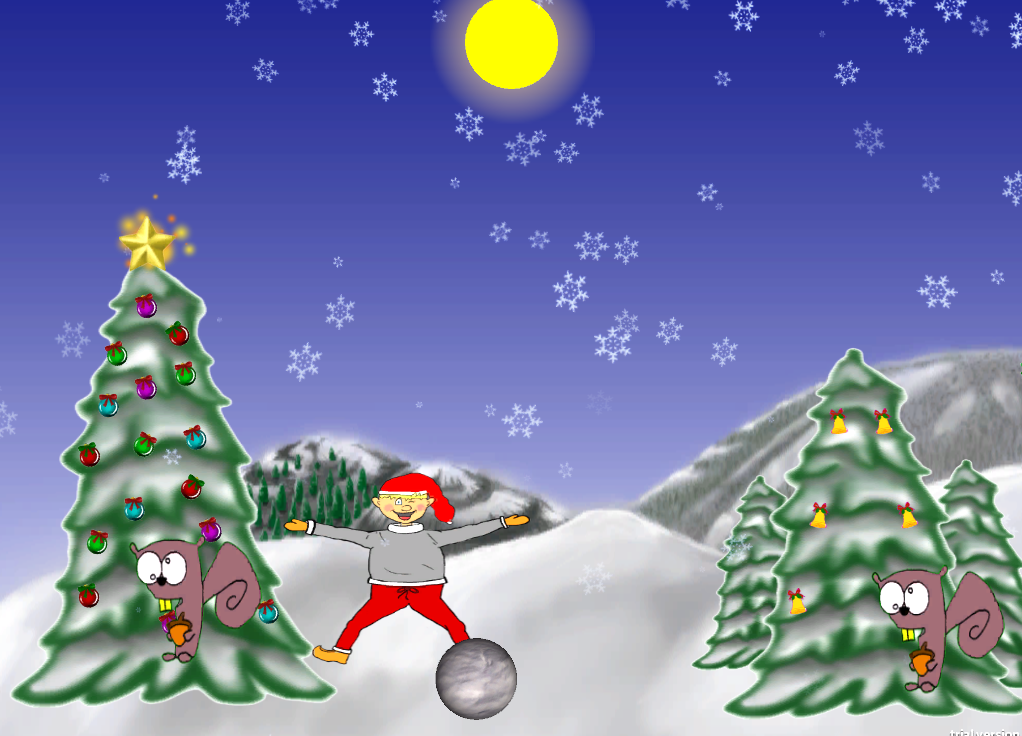
\includegraphics[width=1.00\textwidth]{Pictures/Design/time2.png} %Venstre billede
	\end{minipage}\hfill	
	\begin{minipage}[b]{0.3\textwidth}\centering
		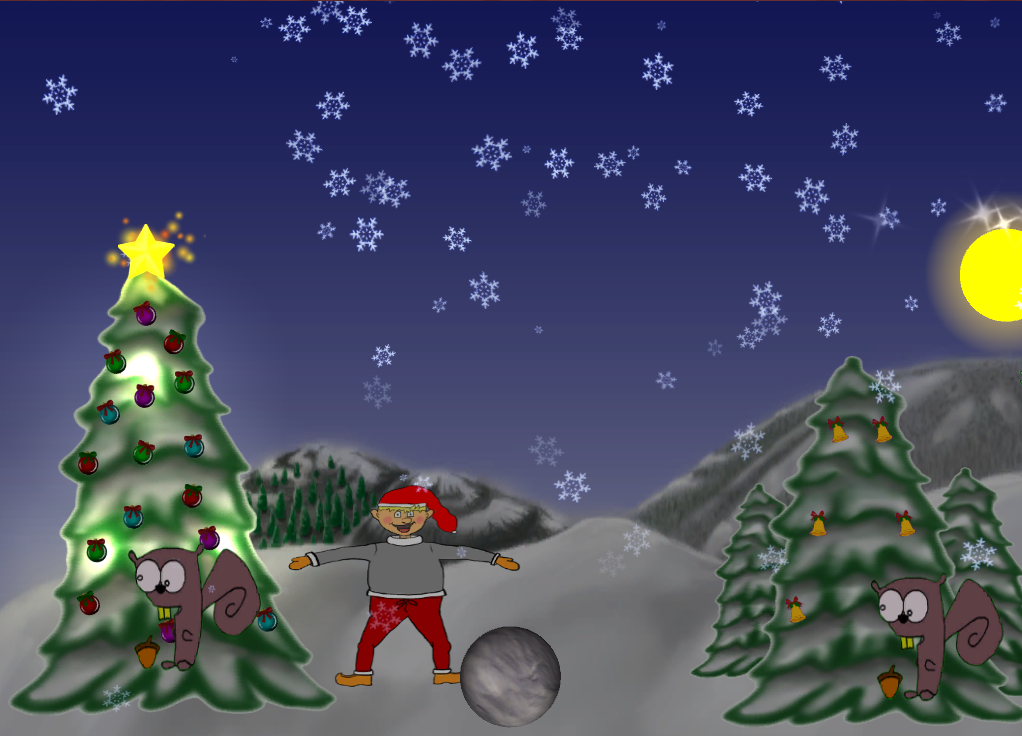
\includegraphics[width=1.00\textwidth]{Pictures/Design/time3.png} %Højre billede
	\end{minipage}\\ %Captions and labels
	\begin{minipage}[t]{0.3\textwidth}
		\caption{Morning.} %Venstre caption og label
		\label{fig:time1}
	\end{minipage}\hfill
	\begin{minipage}[t]{0.3\textwidth}
		\caption{Noon.} %Venstre caption og label
		\label{fig:time2}
	\end{minipage}\hfill	
	\begin{minipage}[t]{0.3\textwidth}
		\caption{Evening.} %Højre caption og label
		\label{fig:time3}
	\end{minipage}
\end{figure}

Another aspect is Santa Claus who will come at a randomly chosen time (see figure \ref{fig:santa}. When he arrives, jingle bell sounds play, as well as his iconic "ho ho ho" laughter. Santa will then drop packages that can be interacted with. This happens by moving into the objects, pushing them with the physics system in Unity. It should be noted that Santa doesn't come too often, since it would disturb other visitors at the library. In average, Santa Claus arrives once an hour.

\begin{figure}[htbp]
\centering
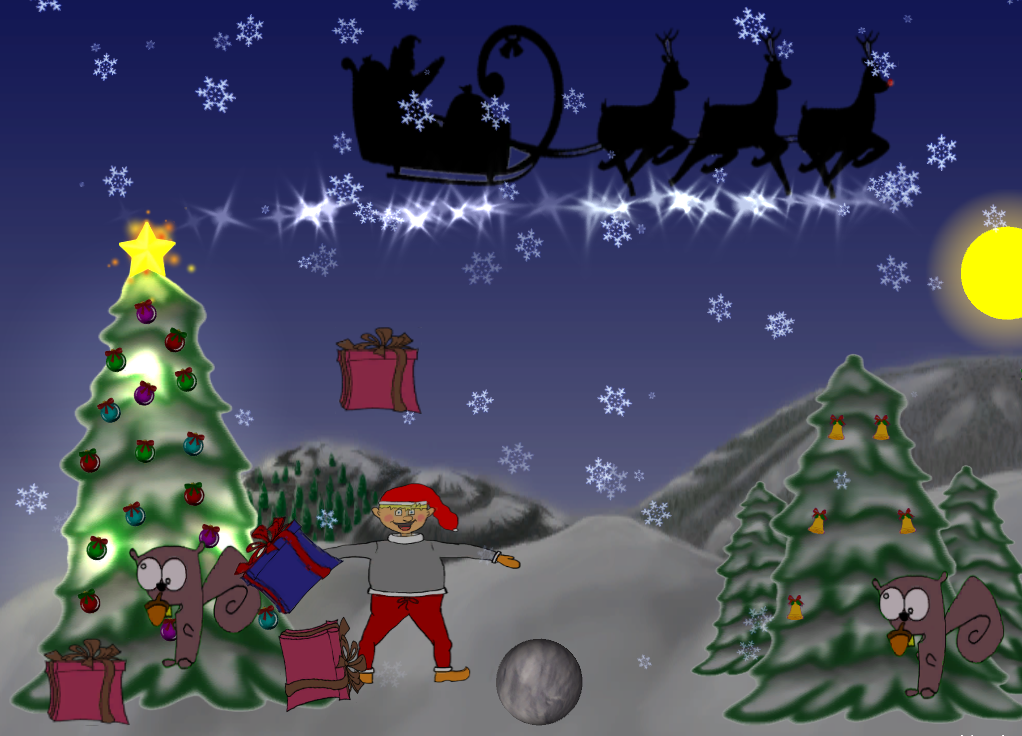
\includegraphics[width=0.90\textwidth]{Pictures/Design/santa.png}
\caption{Santa Claus comes at random times and drop presents. These can be pushed by the characters. They disappear after some time.}
\label{fig:santa}
\end{figure}

\subsection{Snow ball}
To get a little more interaction, a snow ball is placed in the scene (see figure \ref{fig:snowball}). This can be pushed around by the characters, and it will gradually grow bigger and bigger until it at some time explodes and disappear for a short period of time.


\begin{figure}[htbp]
\centering
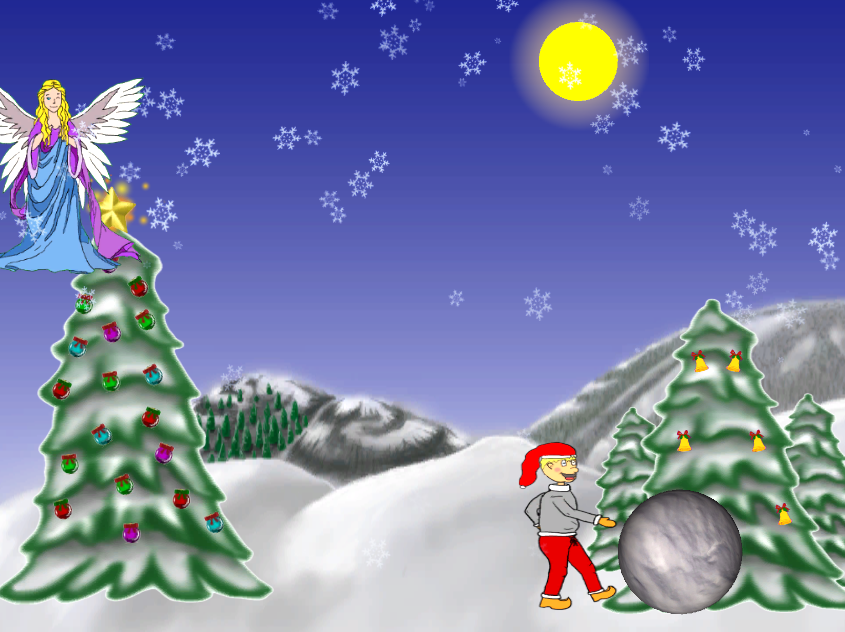
\includegraphics[width=0.90\textwidth]{Pictures/Design/pushing_snowball.png}
\caption{The characters can push the snowball to make it grow. When it becomes big enough, it explodes into colorful fireworks.}
\label{fig:snowball}
\end{figure}
As mentioned in \ref{spritesheet}, sheets of sprites were used to create a sense of motion. This was done by looping over an image containing multiple frames. Depending on which way the character is facing (left, right or idle), the animation will change. Without these animations the whole program would feel rigid and stiff.

\section{Making an automatic batch file}
One of the goals in the problem statement (\ref{problemStatement}) was to have the programs work as easily as possible. We could not expect the library staff to use a lot of time to turn everything on each day. Therefore we wanted everything to start automatically. This was done by creating a batch file that starts when Windows boots up. The batch file then opens the OpenCV program that initializes itself. After 15 seconds Unity opens and starts receiving data from the Clipboard. In the end, the only thing needed is just to turn on (and off) the computer; no additional input is required for the programs to start.

\section{Changes and limitations}
During the setup at the library multiple things were learned. Since it was not possible to be at Hj{\o}rring Library every day, especially not in the beginning of the project, it was difficult to test the proper camera settings, etc. Therefore we needed to re-adjust some elements when we visited the library.

\subsection{Use of LED strips}
The original plan was to be able to track people in front of and behind the bookshelf (dubbed "den r{\o}de tr{\aa}d). Therefore two sets of LED strips was put up: one behind the canvas (see figure \ref{fig:behindShelf}) and one beneath the red bookshelf (see figure \ref{fig:frontShelf}).

What the group hadn't have in mind was that the perspective that the camera would see (figure \ref{fig:camera_POV}). Since the program had already been written without this in mind, it was difficult to make it work with both LED strips. Due to lack of time it was decided to not use the LED strip in the background, but instead solely focus on the LED strip placed underneath the red bookshelf.

One thing that could be interesting to work on in the future would to be the background LED strip recognize hands. When trying out the program, it seemed intuitive to either jump or raise one's arms in the air. The LED strip could be used to track this, so the characters in the program could react accordingly. Sadly, there was no time to implement this idea.

\begin{figure}[htbp] \centering
\begin{minipage}[b]{0.45\textwidth} \centering
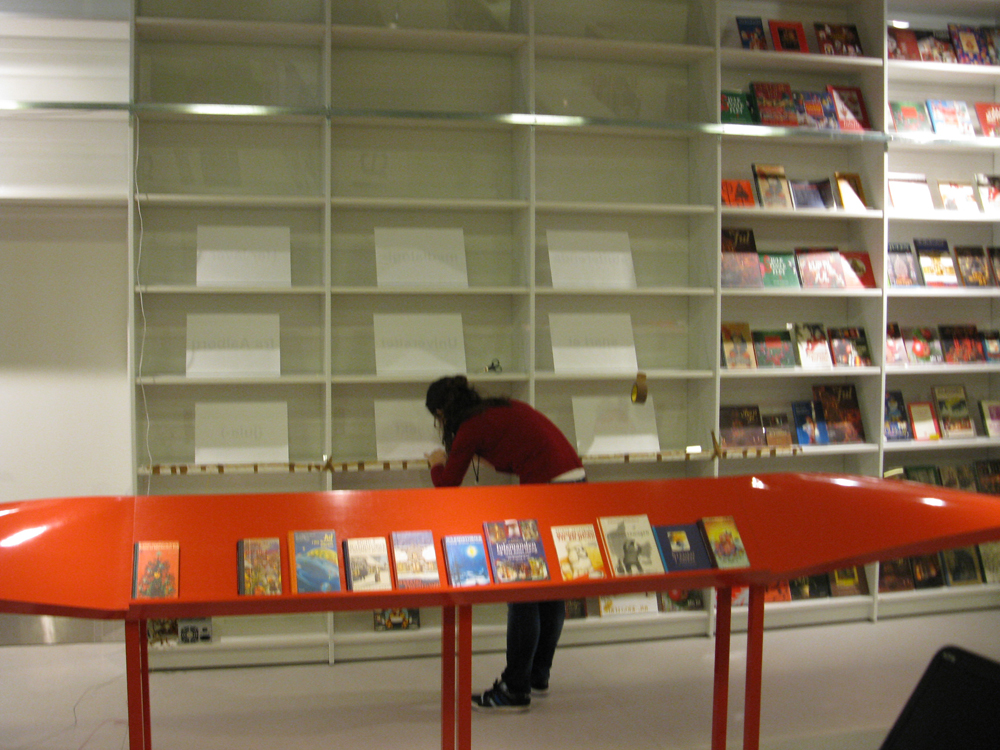
\includegraphics[width=1.00\textwidth]{Pictures/Design/behindShelf} % Venstre billede
\end{minipage} \hfill
\begin{minipage}[b]{0.45\textwidth} \centering
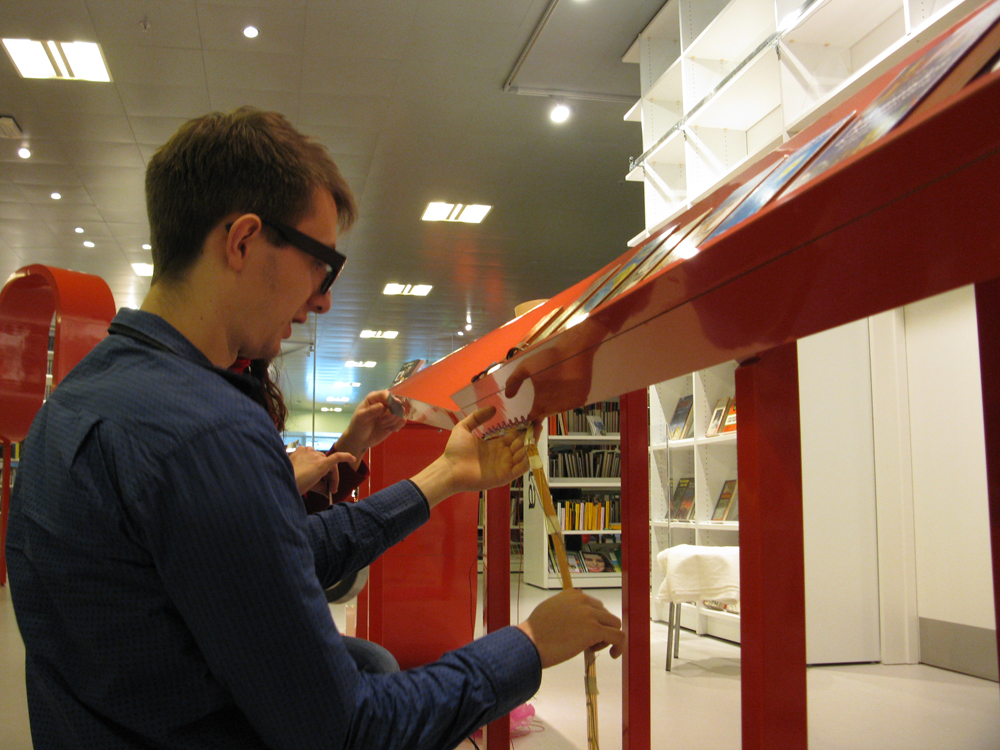
\includegraphics[width=1.00\textwidth]{Pictures/Design/frontShelf} % Højre billede
\end{minipage} \\ % Captions og labels
\begin{minipage}[t]{0.45\textwidth}
\caption{Behind bookshelf.} % Venstre caption og label
\label{fig:behindShelf}
\end{minipage} \hfill
\begin{minipage}[t]{0.45\textwidth}
\caption{Beneah bookshelf} % Højre caption og label
\label{fig:frontShelf}
\end{minipage}
\end{figure}

\begin{figure}[htbp]
\centering
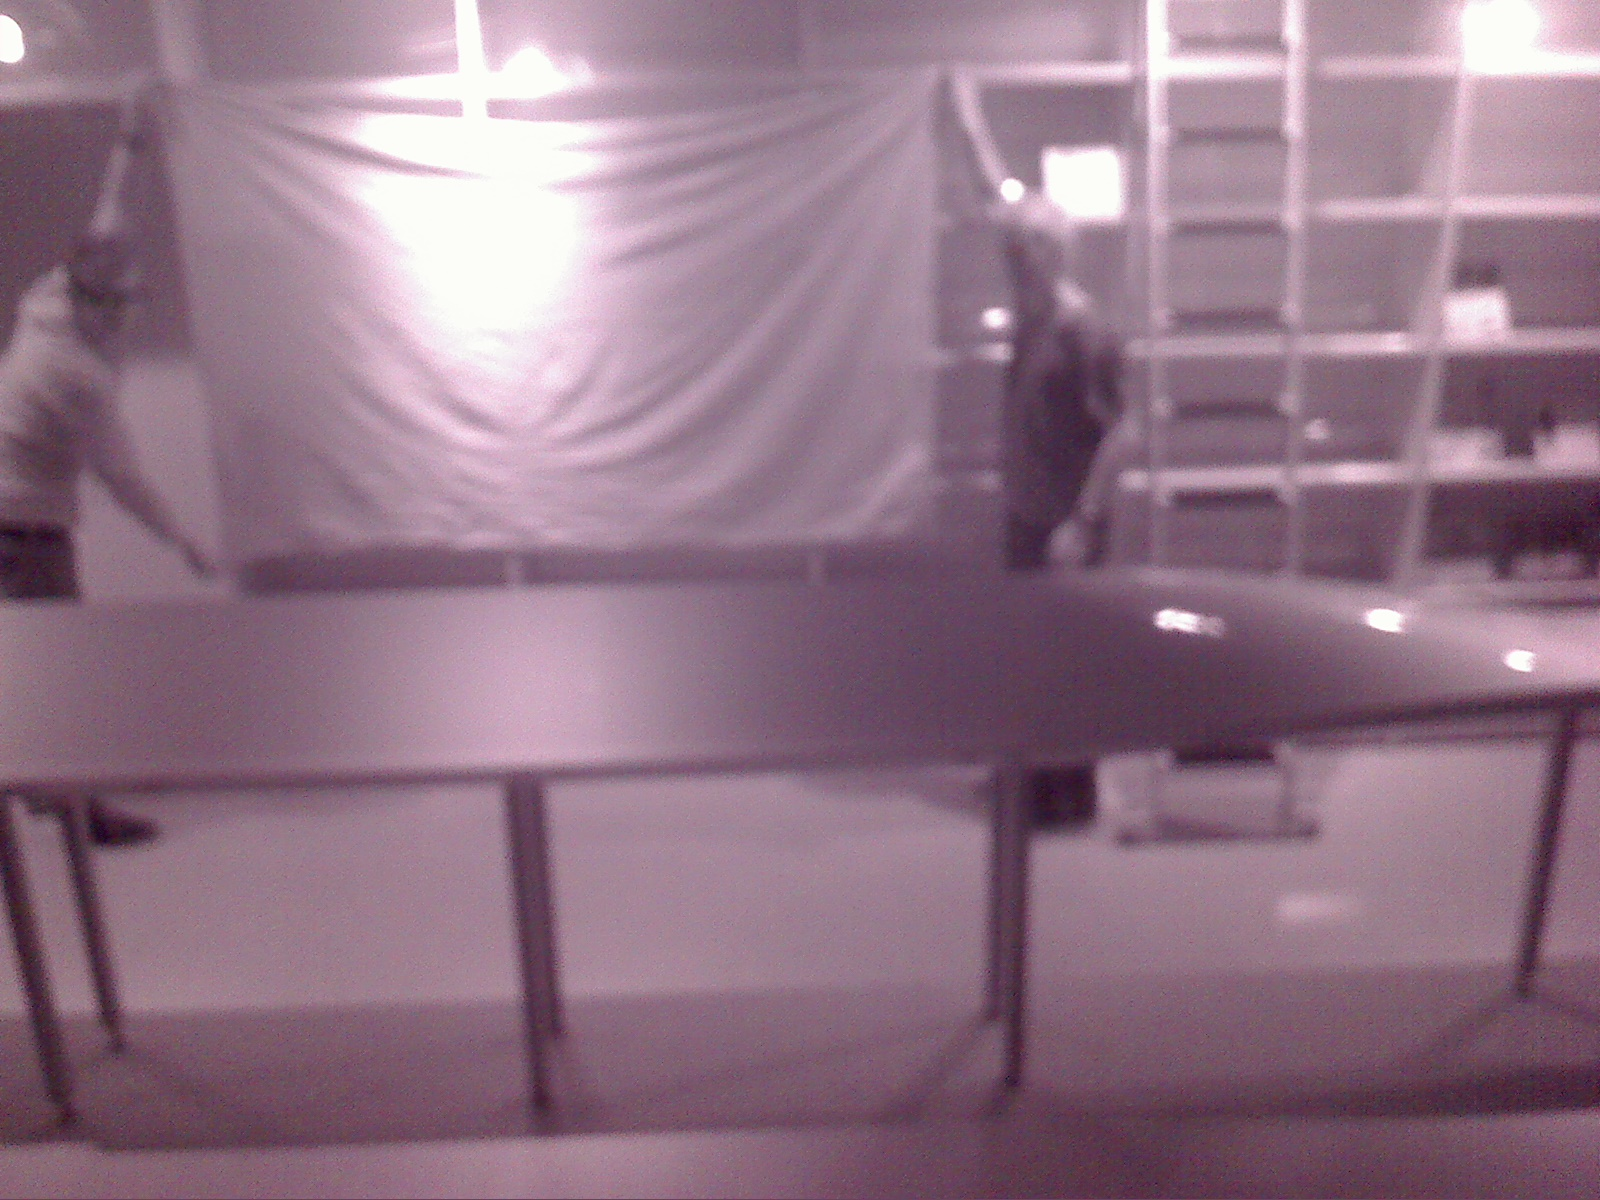
\includegraphics[width=0.70\textwidth]{Pictures/Design/IR_pic}
\caption{Camera point of view.}
\label{fig:camera_POV}
\end{figure}

\subsection{Santa Claus and his "ho ho ho" sound}
As mentioned previously, it was important not to disturb visitors with too much sound. After having the program running for a few hours, one of the library staff members contacted us and asked if it was our program that kept making weird noises. It turned out that she was talking about the Santa Claus "ho ho ho" laughter, which, in her opinion, sounded like a deep and growling voice. Apparently the speakers in that we were using made the "ho ho ho" sound different than on our laptop computers. The staff member said that it was a little disturbing and that she thought kids would be afraid, since it sounded a little creepy. On top of that, it sounded like she was a little annoyed of the sound, since she was working close-by.
In the end the group decided to just get rid of the sound and only use jingle bells for Santa's appearance.

\subsection{Shadows on canvas}
An unexpected problem was the fact that when somebody stand in front of the camera and projector, it draws a rather big shadow on the canvas. When the group first went to Hj{\o}rring to research and look for the location, it didn't seem like it would be a problem.

\textbf{[somebody, Johannes/Simon, needs to write a little more here!]}

\begin{figure}[htbp] \centering
\begin{minipage}[b]{0.45\textwidth} \centering
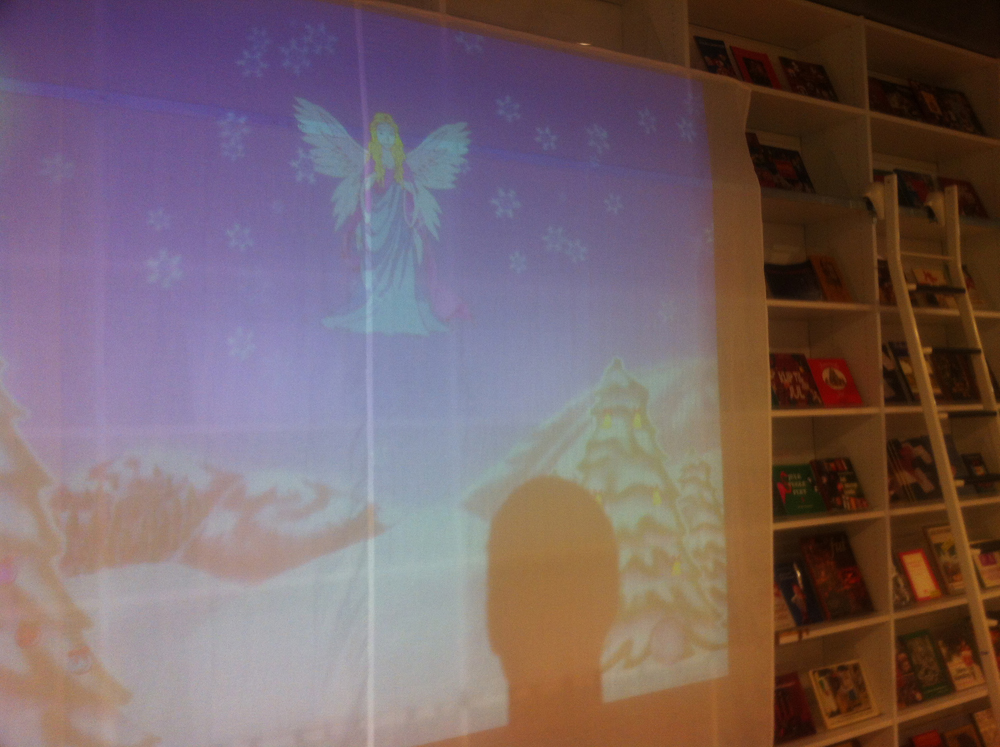
\includegraphics[width=1.00\textwidth]{Pictures/Design/shadow} % Venstre billede
\end{minipage} \hfill
\begin{minipage}[b]{0.45\textwidth} \centering
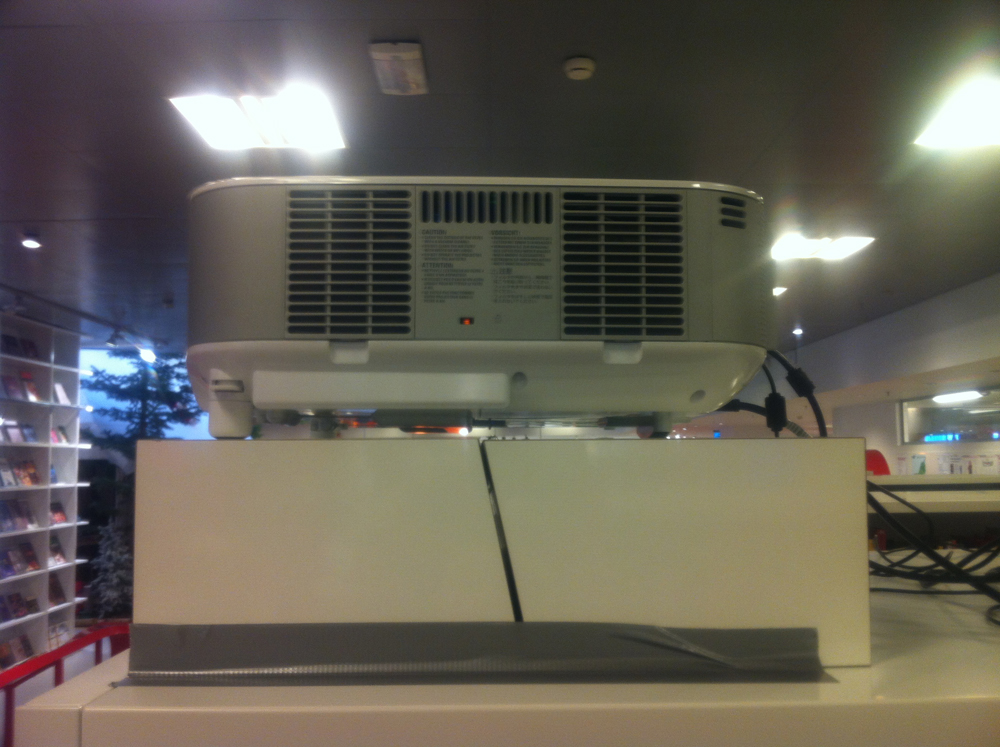
\includegraphics[width=1.00\textwidth]{Pictures/Design/projector_box} % Højre billede
\end{minipage} \\ % Captions og labels
\begin{minipage}[t]{0.45\textwidth}
\caption{If a visitor is standing too close to the red bookshelf, a shadow will cover the canvas.} % Venstre caption og label
\label{fig:shadow_canvas}
\end{minipage} \hfill
\begin{minipage}[t]{0.45\textwidth}
\caption{The projector needed to be placed higher to minimize shadows.} % Højre caption og label
\label{fig:projector_box}
\end{minipage}
\end{figure}

When the final setup was built, it turned out that in the worst-case scenario the shadow would hide a lot of the graphics drawn on the canvas (figure \ref{fig:shadow_canvas}). To reduce the shadows, the projector was placed on top of a couple of boxes (see figure \ref{fig:projector_box}). However, to completely remove the shadows one needed to use a lot of boxes, or, alternatively, hang the projector in the ceiling. Due to time constraints this was not possible. Also, the library staff was afraid that the projector would be too unstable.

\subsection{Need sound to draw attention}
One thing that the group quickly learned while setting the equipment up was the fact that a lot of people didn't even realize the fact that they were interacting with the canvas when the walked past. Many people looked straight forward when they were walking, instead of looking to either sides.

It was suggested to use sounds to draw attention to the canvas. An idea was to make a "magical fairy dust sound" play every time a person stepped into the scene. We tried this, but it didn't give a good result. One reasons was the fact that the speakers are placed inside the projector which is placed in the opposite side of the canvas. Figure \ref{fig:projector_audio} illustrates the problem.

\begin{figure}[htbp]
\centering
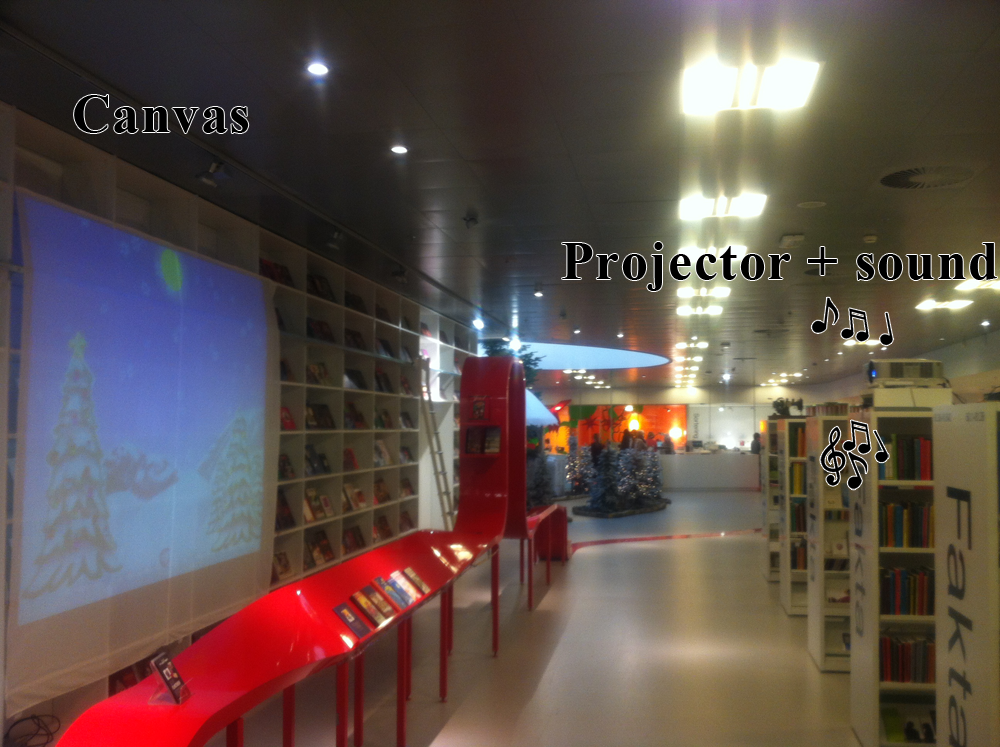
\includegraphics[width=1.0\textwidth]{Pictures/Design/projector_audio}
\caption{Since the speakers are inside the projector, audio will draw attention to the wrong side.}
\label{fig:projector_audio}
\end{figure}

The solution would be to place some external speakers near the canvas, but due to time constraints this wasn't implemented. Also, the sounds turned out to be a little disturbing, so in the end it was chosen to just drop them.

\subsection{People walking too fast}
Another reason why the canvas didn't draw proper attention when people walked past was the fact that it was quite slow to display the characters. In the beginning there was no real connection between a person walking and the character on-screen. This was due to multiple things: the camera having to process the data and send it to Unity, and the speed of the characters. It took some time for the characters to "cath up" on the actual person, so the character would be lagging behind. The solution was to teleport the character if the distance became too big.

\subsection{Camera not steady}
Initially there were some problems with the webcam moving just slightly. This would make the whole program malfunctioning, since the region of interest would change. To avoid this the webcam needed to be steadied with some strong tape. Also, the OpenCV program was modified to re-synchronize itself every hour. This would mean that if somebody accidentally touches either the camera or the LED strips (which happened surprisingly often), the program would re-adjust some time.

The group needed to make a decision: how often should it re-configure itself? If it did it too often, the chances of people standing in front of the camera while it was trying to re-configure was bigger. On the other hand, if it does it less often, the time where it won't work properly would be longer. In the end an hour was chosen to be a good compromise.

\textbf{[MAX should describe more why we chose an hour and not 2 hours, 5 hours, 5 min or something else!?]}

\subsection{Programs crashing during the day}
Before testing the program at the library, they hadn't run for more than a few minutes continuously. Since the goal was to let them run for a whole day (10:00-18:00), it was important that the programs would not crash. Initially, there were problems with both C++ and Unity.

\textbf{[something about C++ crashing]}

Even though the Unity program is quite simple, it turned out to hog a lot of memory over time. It took several days for the group to realize why. After multiple debugging sessions they found that apparently Unity does not deleted old textures and materials. As mentioned earlier, animations are done using sprite sheets. Doing this changes the material on a game object (a material describes how a texture should be displayed using a shader). Every time a new material is applied, i.e. when the animation needed to change, the old material was kept in the background. Over time, these materials stacked up. This meant that the RAM usage constantly increased until the program finally crashed.

To resolve this problem proper deletion of the materials were implemented. It turned out that the {C\#} garbage collector didn't do this automatically, so we manually had to delete old instances of materials. This lead to more stable memory usage. Just to be sure that Unity doesn't use too much memory during a whole day, it was made so that it reloads itself every third hour. This only takes a fraction of a second, so it shouldn't disturb the interaction.
